\documentclass[11pt]{article}

\usepackage[a4paper]{geometry}
\geometry{left=2.0cm,right=2.0cm,top=2.5cm,bottom=2.5cm}

\usepackage{ctex} % 支持中文的LaTeX宏包
\usepackage{amsmath,amsfonts,graphicx,subcaption,amssymb,bm,amsthm,mathrsfs,mathtools,breqn} % 数学公式和符号的宏包集合
\usepackage{siunitx} % SI单位的宏包
\usepackage{algorithm,algorithmicx} % 算法和伪代码的宏包
\usepackage[noend]{algpseudocode} % 算法和伪代码的宏包
\usepackage{fancyhdr} % 自定义页眉页脚的宏包
\usepackage[framemethod=TikZ]{mdframed} % 创建带边框的框架的宏包
\usepackage{fontspec} % 字体设置的宏包
\usepackage{adjustbox} % 调整盒子大小的宏包
\usepackage{fontsize} % 设置字体大小的宏包
\usepackage{tikz} % 绘制图形和使用颜色的宏包
\usepackage{pgfplots} % 绘制数据图表的宏包
\pgfplotsset{compat=1.17} % 设置pgfplots版本兼容性
\usetikzlibrary{arrows.meta,positioning} % TikZ箭头库和定位库
\usepackage{float} % 支持[H]浮动体位置参数
\usepackage{multicol} % 多栏排版的宏包
\usepackage{multirow} % 表格中合并单元格的宏包
\usepackage{pdfpages} % 插入PDF文件的宏包
\RequirePackage{listings} % 在文档中插入源代码的宏包
\usepackage{wrapfig} % 文字绕排图片的宏包
\usepackage{bigstrut,multirow,rotating} % 支持在表格中使用特殊命令的宏包
\usepackage{booktabs} % 创建美观的表格的宏包
\usepackage{threeparttable} % 支持表格注释的宏包
\usepackage{circuitikz} % 绘制电路图的宏包
\usepackage{hyperref} % 创建超链接的宏包
\hypersetup{colorlinks=true, linkcolor=blue, citecolor=blue, urlcolor=blue, bookmarksnumbered=true}
\usepackage[inline]{enumitem} % 自定义列表格式的宏包，支持行内列表

\definecolor{dkgreen}{rgb}{0,0.6,0}
\definecolor{gray}{rgb}{0.5,0.5,0.5}
\definecolor{mauve}{rgb}{0.58,0,0.82}
\lstset{
  frame=tb,
  aboveskip=3mm,
  belowskip=3mm,
  showstringspaces=false,
  columns=flexible,
  framerule=1pt,
  rulecolor=\color{gray!35},
  backgroundcolor=\color{gray!5},
  basicstyle={\small\ttfamily},
  numbers=none,
  numberstyle=\tiny\color{gray},
  keywordstyle=\color{blue},
  commentstyle=\color{dkgreen},
  stringstyle=\color{mauve},
  breaklines=true,
  breakatwhitespace=true,
  tabsize=3,
}


\usepackage[capitalize]{cleveref}
\Crefname{section}{Section}{Sections}
\Crefname{table}{Table}{Tables}
\crefname{table}{Table.}{Tabs.}

\setmainfont{Palatino Linotype}
\setCJKmainfont{SimSun}[BoldFont=SimHei, ItalicFont=KaiTi]
\setCJKsansfont{SimHei}
\setCJKmonofont{FangSong}
\punctstyle{kaiming}
% 偏好的几个字体, 可以根据需要自行加入字体ttf文件并调用

% Restore standard emphasis to avoid requiring an undefined environment (kaishu).
% The original redefinition used an environment `kaishu` which is not defined
% in a default ctex setup and causes compilation errors. Use \textit for
% emphasis which works across engines.
\renewcommand{\emph}[1]{\textit{#1}}

%改这里可以修改实验报告表头的信息
\newcommand{\experiName}{电子荷质比和弗兰克-赫兹实验}
\newcommand{\supervisor}{黄海诺}
\newcommand{\name}{邓思豪}
\newcommand{\studentNum}{2023K8009909008}
\newcommand{\class}{3}
\newcommand{\group}{01}
\newcommand{\seat}{5}
\newcommand{\dateYear}{2025}
\newcommand{\dateMonth}{12}
\newcommand{\dateDay}{17}
\newcommand{\room}{西实208}
\newcommand{\others}{$\square$}


\begin{document}



\begin{center}
    \LARGE \bf 《\, 基\, 础\, 物\, 理\, 实\, 验\, 》\, 实\, 验\, 报\, 告
\end{center}

\begin{center}
    \noindent \emph{实验名称}\underline{\makebox[25em][c]{\experiName}}
    \emph{指导教师}\underline{\makebox[8em][c]{\supervisor}}\\
    \emph{姓名}\underline{\makebox[6em][c]{\name}} 
    % 如果名字比较长, 可以修改box的长度"6em"
    \emph{学号}\underline{\makebox[10em][c]{\studentNum}}
    \emph{分班分组及座号} \underline{\makebox[5em][c]{\class \ -\ \group \ -\ \seat }\emph{号}} （\emph{例}:\, 1\,-\,04\,-\,5\emph{号}）\\
    \emph{实验日期} \underline{\makebox[3em][c]{\dateYear}}\emph{年}
    \underline{\makebox[2em][c]{\dateMonth}}\emph{月}
    \underline{\makebox[2em][c]{\dateDay}}\emph{日}
    \emph{实验地点}\underline{\makebox[6em][c]{\room}}
    \emph{调课/补课} \underline{\makebox[3em][c]{\others\ 是}}
    \emph{成绩评定} \underline{\hspace{5em}}
    {\noindent}
    \rule[8pt]{17cm}{0.2em}
\end{center}

\section{实验目的}
本部分整合弗兰克-赫兹实验与电子荷质比实验的核心目标，具体如下：

\subsection{弗兰克-赫兹实验}
1. 理解弗兰克-赫兹实验通过伏安法验证原子能级量子化的原理与实验方法；
2. 利用弗兰克-赫兹仪记录板极电流与加速电压的关系数据，通过作图计算氩原子的第一激发电位；
3. 学习示波器的基本操作，通过示波器观察板极电流与加速电压的特性曲线，直观认识原子能量的量子化特性。

\subsection{电子荷质比实验}
1. 研究电子在电场中的偏转规律，测量电偏转灵敏度，分析阳极电压对电偏转灵敏度的影响；
2. 研究电子在磁场中的偏转规律，测量磁偏转灵敏度，探讨阳极电压对磁偏转灵敏度的影响；
3. 理解电子透镜的聚焦原理，完成电子束的电聚焦实验，计算不同阳极电压下的聚焦电压比值；
4. 基于磁聚焦原理，测量电子的荷质比（$e/m$），掌握相关实验数据的处理方法；
5. 熟悉电子束测试仪的结构与操作，理解电场、磁场对电子运动的调控机制。

\section{实验仪器与用具 }
\subsection{弗兰克-赫兹实验}
\begin{itemize}
    \item FD-FH-C 微机型弗兰克-赫兹实验仪（含双栅柱面型四极式充氩弗兰克-赫兹管）
    \item 数字存储示波器
    \item BNC 电缆（2根）
\end{itemize}

\begin{figure}[hbtp]
    \centering
    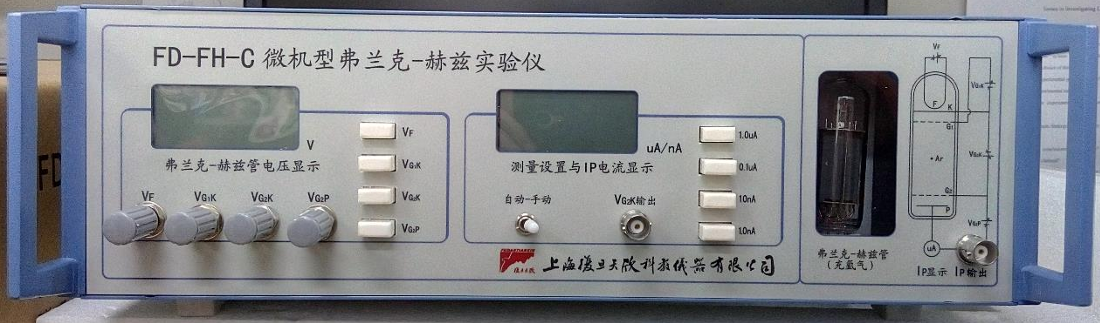
\includegraphics[width=0.8\linewidth]{fh_apparatus.png} % 替换为弗兰克-赫兹实验仪实物图路径
    \caption{FD-FH-C 微机型弗兰克-赫兹实验仪}
    \label{fig:fh_apparatus}
\end{figure}


\subsection{电子荷质比实验}
\begin{itemize}
    \item DH4521 电子束测试仪（内置电偏转电源、磁偏转电源、磁聚焦电源）
    \item 阴极射线管（含电子枪、偏转板、荧光屏）
    \item 长直螺线管（内置线圈，用于磁聚焦实验）
    \item 专用10芯电缆（连接测试仪与示波管）
\end{itemize}

\begin{figure}[hbtp]
    \centering
    \begin{subfigure}[b]{0.45\textwidth}
        \centering
        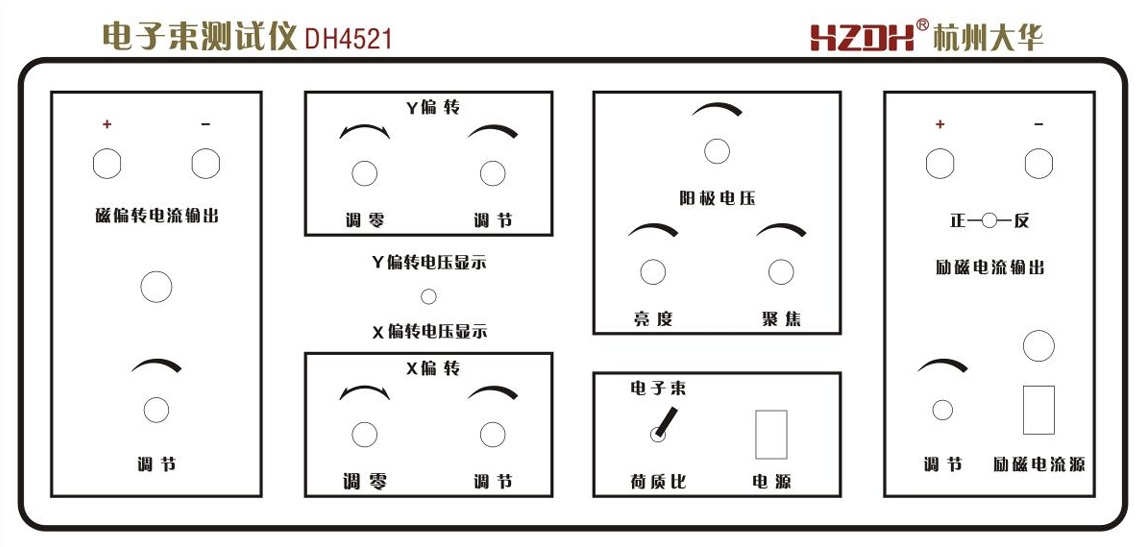
\includegraphics[width=\linewidth]{em_tester.png} % 替换为DH4521电子束测试仪面板图路径
        \caption{DH4521 电子束测试仪操作面板}
        \label{fig:em_tester}
    \end{subfigure}
    \hfill
    \begin{subfigure}[b]{0.45\textwidth}
        \centering
        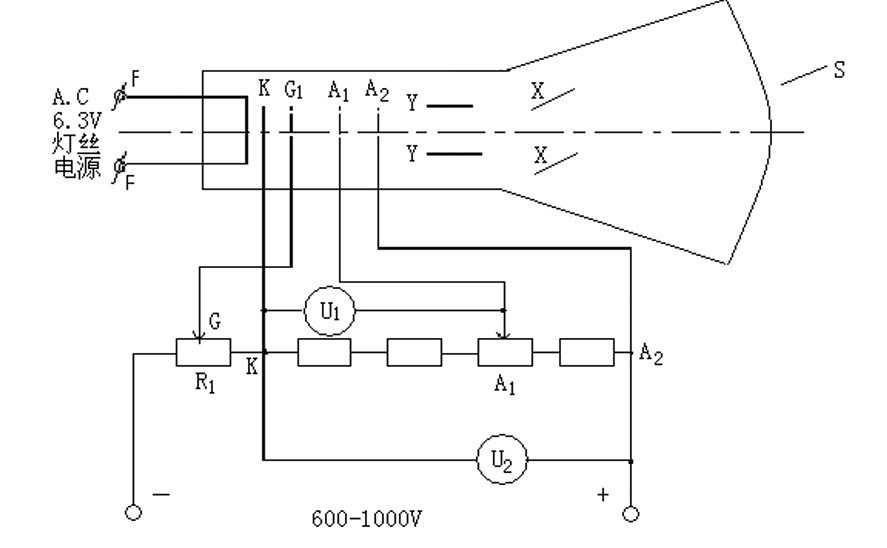
\includegraphics[width=\linewidth]{em_crt.png} % 替换为阴极射线管原理图路径
        \caption{阴极射线管（CRT）结构原理}
        \label{fig:em_crt}
    \end{subfigure}
    \caption{电子荷质比实验核心仪器}
    \label{fig:em_instruments}
\end{figure}

\section{实验原理}
\subsection{电子束的偏转、聚焦与荷质比测量}

\subsubsection{电偏转}
在阴极射线管中，如图\ref{fig:cathode-ray-tube}所示。
\begin{figure}[H]
    \centering
    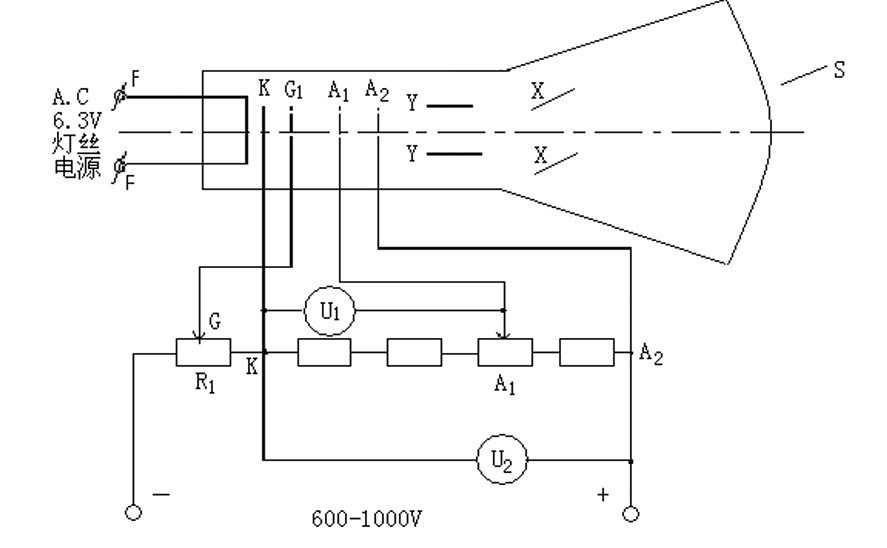
\includegraphics[width=0.8\textwidth]{em_crt.png} % 替换为实际图片文件名
    \caption{阴极射线管原理示意图}
    \label{fig:cathode-ray-tube}
\end{figure}
其中，K为阴极，G为栅极，$A_1$为聚焦阳极，$A_2$为第二阳极，Y为垂直偏转板，X为水平偏转板，S为荧光屏。阴极被灯丝加热发射电子，电子受阳极电场加速；栅极电位可控制电子数，进而调节荧光屏辉度。

电子从阴极发射时初速度近似为0，阳极$A_2$相对阴极的加速电位$U_2$使电子获得轴向速度$v$，由能量关系：
\begin{equation}
    \frac{1}{2}mv^2 = eU_2 \implies v = \sqrt{\frac{2eU_2}{m}}
\end{equation}

电子以速度$v$进入间距为$d$、加电压$U_d$的平行偏转板，板间电场强度$E = \frac{U_d}{d}$，方向与$v$垂直（如图\ref{fig:deflection-plate}）。设板长为$l$，电子通过板的时间$t = \frac{l}{v}$，则$Y$方向加速度$a_y = -\frac{eE}{m}$（负号表示方向与电场相反），电子射出板时的$Y$向偏移量：
\begin{align}
    y_1 &= \frac{1}{2}a_y t^2 = \frac{1}{2}\cdot\frac{eE}{m}\cdot t^2 \\
\intertext{代入 $t = \frac{l}{v}$ 及 $v = \sqrt{\frac{2eU_2}{m}}$，得：}
    y_1 &= \frac{1}{4}\cdot\frac{U_d l^2}{U_2 d}
\end{align}

电子在荧光屏的总偏转量$D = y_1 + L\tan\theta$，其中$\tan\theta = \frac{v_y}{v_z} = \frac{U_d l}{2U_2 d}$，最终得：
\begin{equation}
    D = \frac{1}{2}\cdot\frac{U_d l}{U_2 d}\left(\frac{l}{2} + L\right)
\end{equation}
偏转量$D$随$U_d$增大而增大，与$\frac{l}{2}+L$成正比，与$U_2$、$d$成反比。

\subsubsection{磁偏转}
电子通过$A_2$后，若在垂直于$z$轴方向加均匀磁场，电子受洛伦兹力$F = eBv$（大小不变、方向垂直速度），做匀速圆周运动，洛伦兹力为向心力：
\begin{equation}
    evB = \frac{mv^2}{R} \implies R = \frac{mv}{eB}
\end{equation}
电子离开磁场后沿切线飞向荧光屏。


\subsubsection{电聚焦}
电子射线束的聚焦是所有射线管如示波管、显象管和电子显微镜等都必须解决的问题。在阴极射线管中，阳极被灯丝加热发射电子。电子受阳极产生的正电场作用而加速运动，同时又受栅极产生的负电场作用只有一部分电子能通过栅极小孔而飞向阳极。改变栅极电位能控制通过栅极小孔的电子数目，从而控制荧光屏上的辉度。当栅极上的电位负到一定的程度时，可使电子射线截止，辉度为零。 

聚焦阳极和第二阳极是由同轴的金属圆筒组成。由于各电极上的电位不同，在它们之间形成了弯曲的等位面、电力线。这样就使电子束的路径发生弯曲，类似光线通过透镜那样产生了会聚和发散，这种电子组合称为电子透镜。改变电极间的电位分布，可以改变等位面的弯曲程度，从而达到了电子透镜的聚焦。


\subsubsection{磁聚焦和电子荷质比的测量}
示波管无偏转电压时，第二阳极电压$U_2$使电子轴向速度$v_{\parallel} = \sqrt{\frac{2eU_2}{m}}$。给偏转板加交变电压，电子获$v_{\perp}$，荧光屏出现直线；螺线管通电流$I$产生磁场$B$，电子受$F = e v_{\perp} B$做圆周运动，半径$R = \frac{m v_{\perp}}{e B}$，周期：
\begin{equation}
    T = \frac{2\pi R}{v_{\perp}} = \frac{2\pi m}{e B}
\end{equation}

电子轨迹为螺旋线，螺距$h = v_{\parallel} T = \frac{2\pi}{B} \sqrt{\frac{2mU_2}{e}}$（与$v_{\perp}$无关，此为磁聚焦原理）。由$h$的表达式得荷质比：
\begin{equation}
    \frac{e}{m} = \frac{8\pi^2 U_2}{h^2 B^2}
\end{equation}

长直螺线管磁感应强度$B = \frac{\mu_0 N I}{\sqrt{L^2 + D_0^2}}$（$\mu_0 = 4\pi \times 10^{-7}\mathrm{H/m}$），代入得：
\begin{equation}
    \frac{e}{m} = \frac{8\pi^2 U_2 (L^2 + D_0^2)}{(\mu_0 N I h)^2}
  \end{equation}

本仪器参数：
\begin{itemize}
    \item 螺线管匝数：$N = 535 \pm 1$；
    \item 螺线管长度：$L = 0.235\,\mathrm{m}$；
    \item 螺线管直径：$D_0 = 0.092\,\mathrm{m}$；
    \item 螺距（$Y$偏转板至荧光屏距离）：$h = 0.135\,\mathrm{m}$。
\end{itemize}

\subsection{弗兰克-赫兹实验原理}

\subsubsection{电子与原子之间的相互作用}
根据玻尔理论的定态能级假设，原子只能处在一些稳定的状态中，其中每一状态对应一定的能量值 $E_j \ (j = 1, 2, 3, \dots)$，这些数值是彼此分立的、不连续的。根据能级跃迁假设，原子只能吸收和辐射两定态能级差的能量。因此，想要激发处于基态的原子，所提供的能量不能小于基态跃迁到第一激发态时所需的能量。弗兰克-赫兹实验是通过具有一定能量的电子与原子碰撞、进行能量交换，实现原子从基态到高能态的跃迁。

电子与原子碰撞过程的能量守恒关系为：
\begin{equation}
    \frac{1}{2}m_{\text{e}}v^2 + \frac{1}{2}MV^2 = \frac{1}{2}m_{\text{e}}{v'}^2 + \frac{1}{2}M{V'}^2 + \Delta E
\end{equation}
其中：$m_{\text{e}}$ 为电子质量，$M$ 为原子质量，$v/v'$ 为电子碰撞前/后速度，$V/V'$ 为原子碰撞前/后速度，$\Delta E$ 为原子内能变化量。

由于 $m_{\text{e}} \ll M$，电子动能可转化为原子内能；且原子内能不连续：
\begin{itemize}
    \item 当电子动能 $<$ 原子第一激发电位对应的能量时，发生弹性碰撞，$\Delta E = 0$；
    \item 当电子动能 $\geq$ 原子第一激发电位对应的能量时，发生非弹性碰撞，$\Delta E = E_1$（$E_1$ 为原子第一激发电位）。
\end{itemize}

\subsubsection{早期的弗兰克-赫兹实验}
1911年，弗兰克和赫兹改进勒纳的单栅三级式碰撞管结构（缩小加速极G与收集极板P间距、减小减速电压），改用单原子气体（氮、汞）开展实验：汞为单原子分子、常温液态（易控密度）、原子量大（电子碰撞能量损失小）；钾/钠/镁（不易形成负离子）、氩/氖（惰性气体，电子亲和势小）也常用于碰撞规律研究。

\begin{figure}[H]
    \centering
    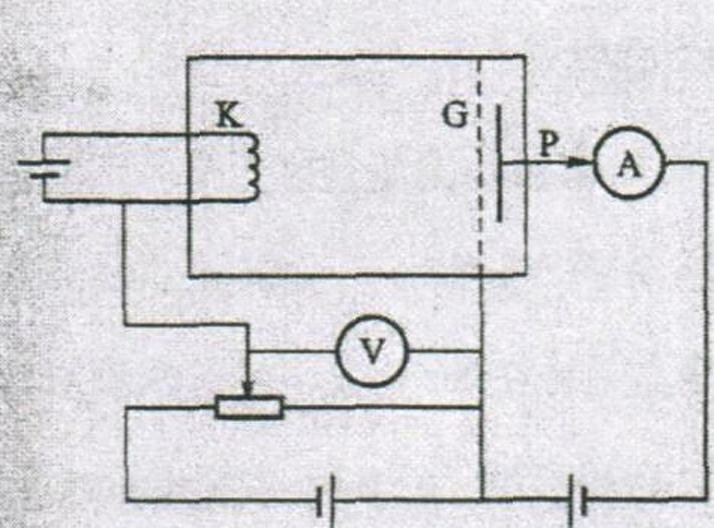
\includegraphics[width=0.5\textwidth]{fig2_1.png} % 替换为图2.1实际文件名
    \caption{早期的弗兰克—赫兹实验装置示意图}
    \label{fig:fh_early_setup}
\end{figure}

1914年，利用图\ref{fig:fh_early_setup}装置得到管流-加速电压关系（图\ref{fig:hg_current_v}）：电子由热阴极K发射，经K-G电场加速后，需克服G-P减速电场才能到达P极形成管流 $I_{\text{P}}$。

\begin{figure}[H]
    \centering
    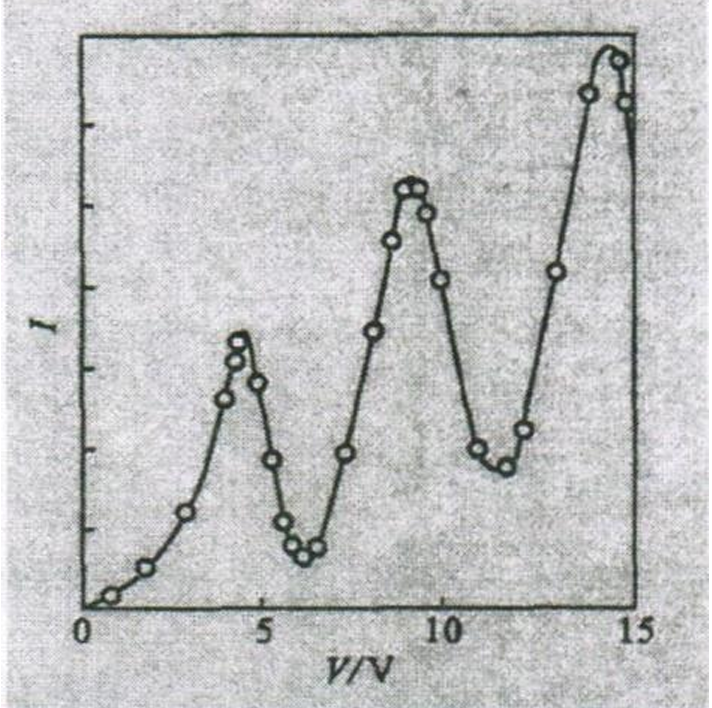
\includegraphics[width=0.4\textwidth]{fig2_2.png} % 替换为图2.2实际文件名
    \caption{早期充汞管得到的管流与加速电压的关系图}
    \label{fig:hg_current_v}
\end{figure}

1920年，弗兰克改进装置（旁热式阴极+新增栅极 $\text{G}_1$+降低汞蒸汽压，图\ref{fig:fh_improved_setup}）：电子在 $\text{K-G}_1$ 加速、$\text{G}_1\text{-G}_2$ 等势区碰撞，可测得汞原子多量子态（汞第一激发能$4.89\,\mathrm{eV}$，对应光谱波长$253.7\,\mathrm{nm}$）。

\begin{figure}[H]
    \centering
    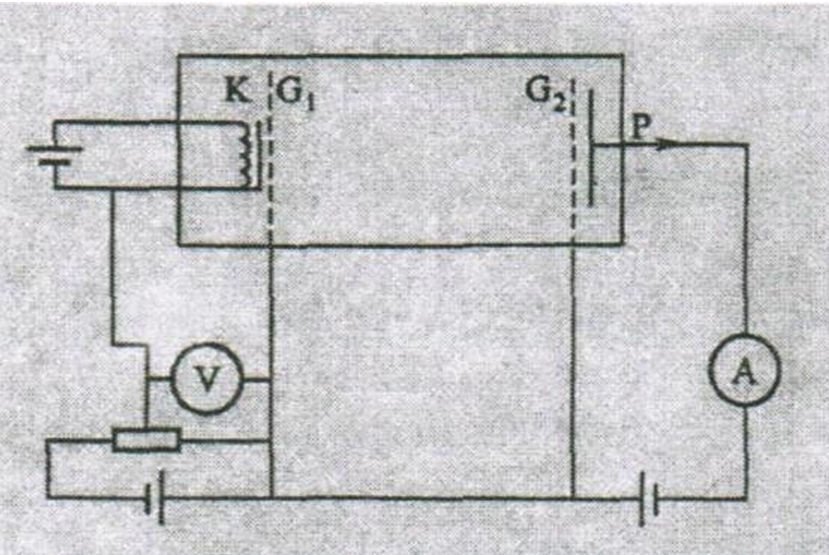
\includegraphics[width=0.5\textwidth]{fig2_3.png} % 替换为图2.3实际文件名
    \caption{改进后的弗兰克—赫兹实验装置示意图}
    \label{fig:fh_improved_setup}
\end{figure}

\subsubsection{双栅柱面型四极式弗兰克-赫兹管}
FD-FH-C型实验仪采用双栅柱面型四极式弗兰克-赫兹管（图\ref{fig:fh_tube_struct}）：板极P为镀铝圆筒，控制栅 $\text{G}_1$、加速栅 $\text{G}_2$ 为钼丝螺旋线，阴极K为镀三元氧化物的镍管，灯丝F为双向绞绕钨丝（与K构成傍热式阴极）；部件同轴固定后抽真空、充氖气。

\begin{figure}[H]
    \centering
    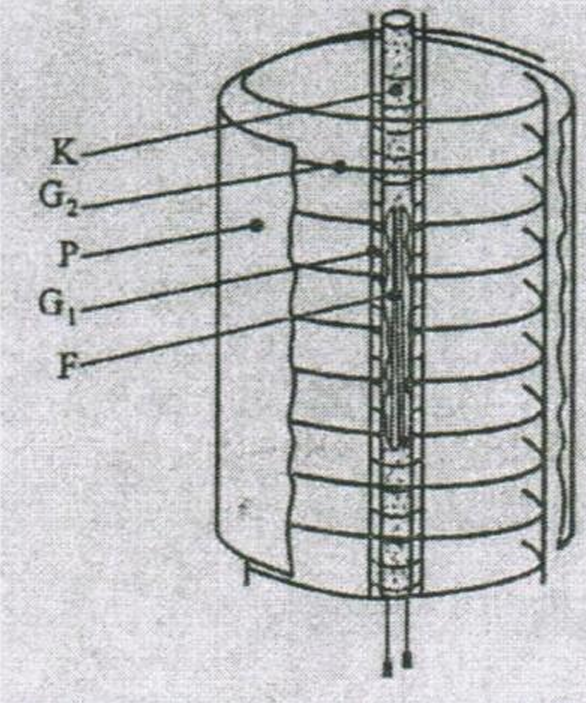
\includegraphics[width=0.4\textwidth]{fig2_4.png} % 替换为图2.4实际文件名
    \caption{复旦双栅柱面型四极式弗兰克—赫兹管结构图}
    \label{fig:fh_tube_struct}
\end{figure}

管内关键电压参数：
\begin{enumerate}[label=(\arabic*)]
    \item 灯丝电压 $V_{\text{F}}$：影响阴极发射系数，低温对应电子速度分布窄、击穿电压高；
    \item 控制栅电压 $V_{\text{G}_1\text{K}}$：消除电子堆积，一般取$1\,\mathrm{V}$左右，需实验选最佳值；
    \item 加速电压 $V_{\text{G}_2\text{K}}$：上限以管子不电离为界，随实验条件变化；
    \item 减速电压 $V_{\text{G}_2\text{P}}$：过滤低能电子，充汞管取$0.5\text{-}2\,\mathrm{V}$、充氖管取$2\text{-}8\,\mathrm{V}$。
\end{enumerate}

\subsubsection{实验装置原理}
FD-FH-C型仪采用充氖弗兰克-赫兹管（图\ref{fig:fh_exp_setup}）：电子经 $\text{K-G}_1$ 加速后，在 $\text{G}_1\text{G}_2$ 区与氖原子碰撞；能量 $> e V_{\text{G}_2\text{P}}$ 的电子可克服 $\text{G}_2\text{-P}$ 减速电场到达P极，形成板流 $I_{\text{P}}$。

\begin{figure}[H]
    \centering
    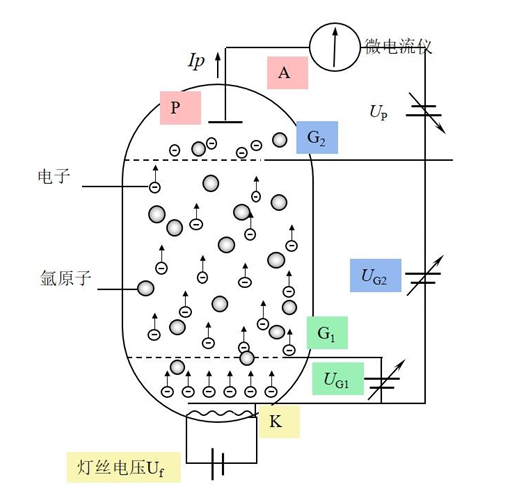
\includegraphics[width=0.7\textwidth]{fig2_5.png} % 替换为图2.5实际文件名
    \caption{弗兰克—赫兹实验装置示意图}
    \label{fig:fh_exp_setup}
\end{figure}

随 $V_{\text{G}_2\text{K}}$ 增大，电子能量升高：
\begin{itemize}
    \item 能量不足时，碰撞后无法到达P极，$I_{\text{P}}$ 下降；
    \item 能量足够时，$I_{\text{P}}$ 上升；
    \item 能量达 $2\Delta E$ 时，二次非弹性碰撞使 $I_{\text{P}}$ 二次下降。
\end{itemize}

多次碰撞使 $I_{\text{P}}\text{-}V_{\text{G}_2\text{K}}$ 曲线呈现周期性下降（图\ref{fig:ne_current_v}），相邻峰/谷的 $V_{\text{G}_2\text{K}}$ 差即为氖原子第一激发电位，证明原子能量状态的不连续性。

\begin{figure}[H]
    \centering
    \begin{subfigure}[b]{0.45\textwidth}
        \centering
        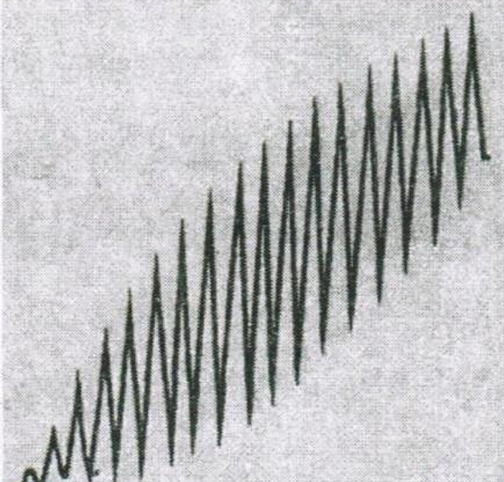
\includegraphics[width=\textwidth]{fig2_6a.png} % 替换为图2.6(a)实际文件名
        \caption{汞第一激发能态曲线}
    \end{subfigure}
    \hfill
    \begin{subfigure}[b]{0.45\textwidth}
        \centering
        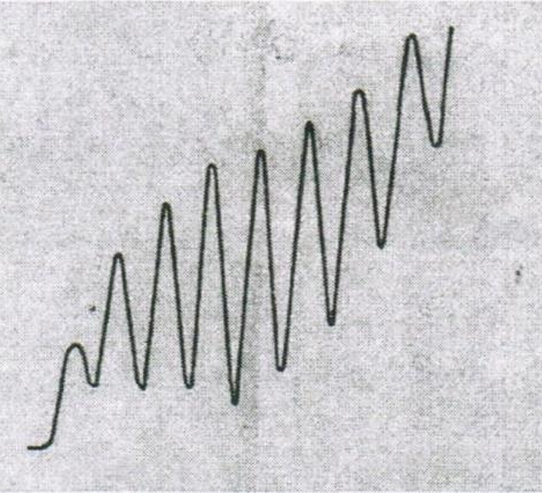
\includegraphics[width=\textwidth]{fig2_6b.png} % 替换为图2.6(b)实际文件名
        \caption{氖第一激发能态曲线}
        \label{fig:ne_current_v}
    \end{subfigure}
    \caption{第一激发能态曲线对比}
\end{figure}

\section{实验步骤}
\subsection{电子束实验}
\subsubsection{电偏转}
实验装置仪器面板如图\ref{fig:device_panel}所示：

\begin{figure}[H]
    \centering
    
\includegraphics[width=0.8\textwidth]{fig3.png} % 替换为图3实际文件路径
    \caption{设备操作面板图}
    \label{fig:device_panel}
\end{figure}

\begin{enumerate}
    \item 先用专用10芯电缆连接测试仪和示波管，再开启电源开关，将“电子束—荷质比”选择开关打向电子束位置，辉度适当调节，并调节聚焦，使屏上光点聚成一细点。应注意：光点不能太亮，以免烧坏荧光屏。
    \item 光点调零：将面板上钮子开关打向$X$偏转电压显示，调节“$X$调节”旋钮，使电压表的指针在零位，再调节$X$调零旋钮，使光点位于示波管垂直中线上；同$X$调零一样，将面板上钮子开关打向$Y$偏转电压显示，将$Y$调节后，光点位于示波管的中心原点。
    \item 测量偏转量 $D$ 随电偏转电压 $U_d$ 变化：调节阳极电压旋钮，给定阳极电压 $U_2$。将电偏转电压表显示打到显示$Y$偏转调节（垂直电压），改变 $U_d$ 测一组 $D$ 值。改变 $U_2$ 后再测 $D\text{-}U_d$ 变化（$U_2$：$600\text{-}1000\,\mathrm{V}$）。
    \item 求$Y$轴电偏转灵敏度 $D/U_d$，并说明为什么 $U_2$ 不同，$D/U_d$ 不同。
    \item 同$Y$轴一样，也可以测量$X$轴的电偏转灵敏度。
\end{enumerate}
\subsubsection{磁偏转}
依照图\ref{fig:exp_step_fig4}完成以下步骤：

\begin{figure}[H]
    \centering
    
\includegraphics[width=0.8\textwidth]{fig4.png} % 请替换为图4实际文件路径
    \caption{实验装置连接示意图}
    \label{fig:exp_step_fig4}
\end{figure}

\begin{enumerate}
    \item 开启电源开关，将“电子束—荷质比”选择开关打向电子束位置，辉度适当调节，并调节聚焦，使屏上光点聚成一细点，应注意：光点不能太亮，以免烧坏荧光屏。
    \item 光点调零：通过调节“$X$调节”和“$Y$调节”旋钮，使光点位于$Y$轴的中心原点。
    \item 测量偏转量 $D$ 随磁偏转电流 $I$ 的变化：给定 $U_2$，将磁偏转电流输出与磁偏转电流输入相连，调节磁偏转电流调节旋钮（改变磁偏转线圈电流的大小）测量一组 $D$ 值。改变磁偏转电流方向，再测一组 $D\text{-}I$ 值。改变 $U_2$，再测两组 $D\text{-}I$ 数据（$U_2$：$600\text{-}1000\,\mathrm{V}$）。通过钮子开关切换磁偏转电流方向，再次实验。
    \item 求磁偏转灵敏度 $D/I$，并解释为什么 $U_2$ 不同，$D/I$ 不同。
\end{enumerate}
\subsubsection{电聚焦}
依照图\ref{fig:exp_fig3}完成以下步骤：

\begin{figure}[H]
    \centering
    
\includegraphics[width=0.8\textwidth]{fig3.png} % 请替换为图3实际文件路径
    \caption{实验装置操作面板图}
    \label{fig:exp_fig3}
\end{figure}

\begin{enumerate}
    \item 开启电源开关，将“电子束—荷质比”选择开关打向电子束位置，辉度适当调节，并调节聚焦，使屏上光点聚成一细点，应注意：光点不能太亮，以免烧坏荧光屏。
    \item 光点调零：通过调节“$X$调节”和“$Y$调节”旋钮，使光点位于$Y$轴的中心原点。
    \item 调节阳极电压 $U_2$ 分别为 $600\text{-}1000\,\mathrm{V}$，对应的调节聚焦旋钮（改变聚焦电压）使光点达到最佳的聚焦效果，测量出各对应的聚焦电压 $U_1$。
    \item 求出 $U_2/U_1$。
\end{enumerate}
\subsubsection{磁聚焦与电子荷质比测量}
依照图\ref{fig:exp_fig6}完成以下步骤：

\begin{figure}[H]
    \centering
    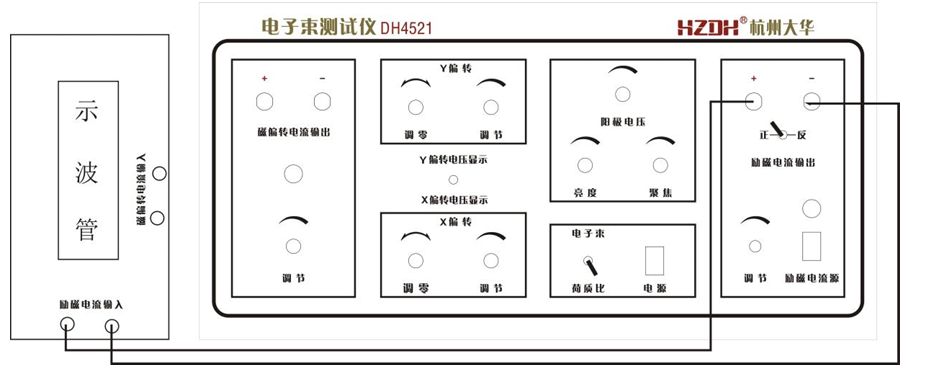
\includegraphics[width=0.8\textwidth]{fig6.png} % 请替换为图六实际文件路径
    \caption{电子束测试仪实验连接示意图}
    \label{fig:exp_fig6}
\end{figure}

\begin{enumerate}
    \item 开启电子束测试仪电源开关，“电子束——荷质比”开关置于荷质比方向，此时荧光屏上出现一条直线，阳极电压调到 $700\,\mathrm{V}$。
    \item 将励磁电流部分的调节旋钮逆时针方向调节到头，并将励磁电流输出与励磁电流输入相连（螺线管）。
    \item 电流换向开关打向正向，调节输出调节旋钮，逐渐加大电流使荧光屏上的直线一边旋转一边缩短，直到出现第一个小光点，读取此时对应的电流值 $I_{\text{正}}$，然后将电流调为零。再将电流换向开关打向反向（改变螺线管中磁场方向），重新从零开始增加电流使屏上的直线反方向旋转并缩短，直到再得到一个小光点，读取此时电流值 $I_{\text{反}}$。
    \item 改变阳极电压为 $800\,\mathrm{V}$，重复步骤3，直到阳极电压调到 $1000\,\mathrm{V}$ 为止。
    \item 数据记录和处理：
    将所测各数据记入表中，通过式
    \begin{equation}
        \frac{e}{m} = \frac{8\pi^2 U_2 (L^2 + D_0^2)}{(\mu_0 N I h)^2}
    \end{equation}
    计算出电子荷质比 $e/m$。
\end{enumerate}
\subsection{弗兰克-赫兹实验}

\subsubsection{手动测量法}
\begin{enumerate}
    \item 调节 $V_{\text{G}_2\text{K}}$ 至最小，扫描开关置于“手动”档，打开主机电源。
    \item 分别调节 $V_{\text{F}}$、$V_{\text{G}_1\text{K}}$ 和 $V_{\text{G}_2\text{P}}$ 电压（可以先参考仪器给出值）至合适值，将“测量设置”与 $I_{\text{P}}$ 电流显示切换至 $1.0\,\mu\mathrm{A}$ 档，用手动方式逐渐增大 $V_{\text{G}_2\text{K}}$，同时观察 $I_{\text{P}}$ 电流变化，可以看到至少出现 7 个峰。
    \item 选取合适实验点，分别由表头读取 $I_{\text{P}}$ 和 $V_{\text{G}_2\text{K}}$ 值（$I_{\text{P}}$ 电流读数方法为显示值乘以档位，如表头数值 0.342，档位 $1.0\,\mu\mathrm{A}$，则 $I_{\text{P}}$ 电流数值为 $0.342\,\mu\mathrm{A}$，以此类推），作图可得 $I_{\text{P}}\text{-}V_{\text{G}_2\text{K}}$ 曲线。
    \item 由曲线的特征点求出弗兰克—赫兹管中氖原子的第一激发电位。
\end{enumerate}

\subsubsection{示波器观察法}
\begin{enumerate}
    \item 连接好主机后面板电源线，用 BNC 电缆将前面板的“$V_{\text{G}_2\text{K}}$ 输出”与示波器上的通道 1 ($X$) 连接，“$I_{\text{P}}$ 输出”与示波器的通道 2 ($Y$) 连接，将示波器扫描开关置于“自动”档。
    \item 打开示波器（数字存储示波器），将示波器设置在“Auto”模式。
    \item 打开弗兰克-赫兹实验仪，稍等片刻（弗兰克-赫兹管需要预热）。
    \item 分别调节 $V_{\text{F}}$、$V_{\text{G}_1\text{K}}$、$V_{\text{G}_2\text{P}}$ 电压至合适数值（参考仪器给出的合适值），将测量 $I_{\text{P}}$ 电流显示切换至 $1.0\,\mu\mathrm{A}$ 档，用手动方式逐渐增大 $V_{\text{G}_2\text{K}}$（注意不要击穿弗兰克-赫兹管），直至示波器上出现稳定的 $I\text{-}V$ 特性曲线，观察原子能量的量子化情况。
\end{enumerate}

\section{实验数据和处理}
\subsection{电偏转实验数据}
\begin{table}[H]
\centering
\caption{电子束电偏转灵敏度数据记录表}
\label{tab:elec_deflection}
\footnotesize
\setlength{\tabcolsep}{3pt}
\begin{tabular}{cccccccc}
\toprule
\multicolumn{4}{c}{阳极电压 $U_2 = 600$ V} & \multicolumn{4}{c}{阳极电压 $U_2 = 700$ V} \\
\cmidrule(lr){1-4} \cmidrule(lr){5-8}
\multicolumn{2}{c}{方向 X} & \multicolumn{2}{c}{方向 Y} & \multicolumn{2}{c}{方向 X} & \multicolumn{2}{c}{方向 Y} \\
\cmidrule(lr){1-2} \cmidrule(lr){3-4} \cmidrule(lr){5-6} \cmidrule(lr){7-8}
$U$ (V) & $D$ (mm) & $U$ (V) & $D$ (mm) & $U$ (V) & $D$ (mm) & $U$ (V) & $D$ (mm) \\
\midrule
4.9   & 4   & -4.6  & -5  & 7.6   & 5   & -5.8  & -5  \\
8.0   & 5.5 & -9.6  & -10 & 15.8  & 10  & -11.2 & -10 \\
12.3  & 9   & -14.2 & -15 & 23.0  & 15  & -16.9 & -15 \\
16.4  & 12  & -19.1 & -20 & 31.2  & 20  & -22.2 & -20 \\
20.5  & 15  & -23.7 & -25 & 38.8  & 25  & -27.6 & -25 \\
27.1  & 20  & -28.3 & -30 & 46.6  & 30  & -32.9 & -30 \\
0     & 0   & 0     & 0   & 0     & 0   & 0     & 0   \\
33.6  & 25  & 4.8   & 5   & -8.0  & -5  & 5.2   & 5   \\
40.6  & 30  & 9.4   & 10  & -15.8 & -10 & 10.5  & 10  \\
-7.0  & -5  & 14.0  & 15  & -23.9 & -15 & 15.8  & 15  \\
-13.5 & -10 & 18.2  & 20  & -30.9 & -20 & 21.0  & 20  \\
-20.9 & -15 & 22.5  & 25  & -38.5 & -25 & 25.8  & 25  \\
-27.1 & -20 & 26.6  & 30  & -46.7 & -30 & 30.2  & 30  \\
\bottomrule
\end{tabular}
\end{table}

\begin{figure}[H]
    \centering
    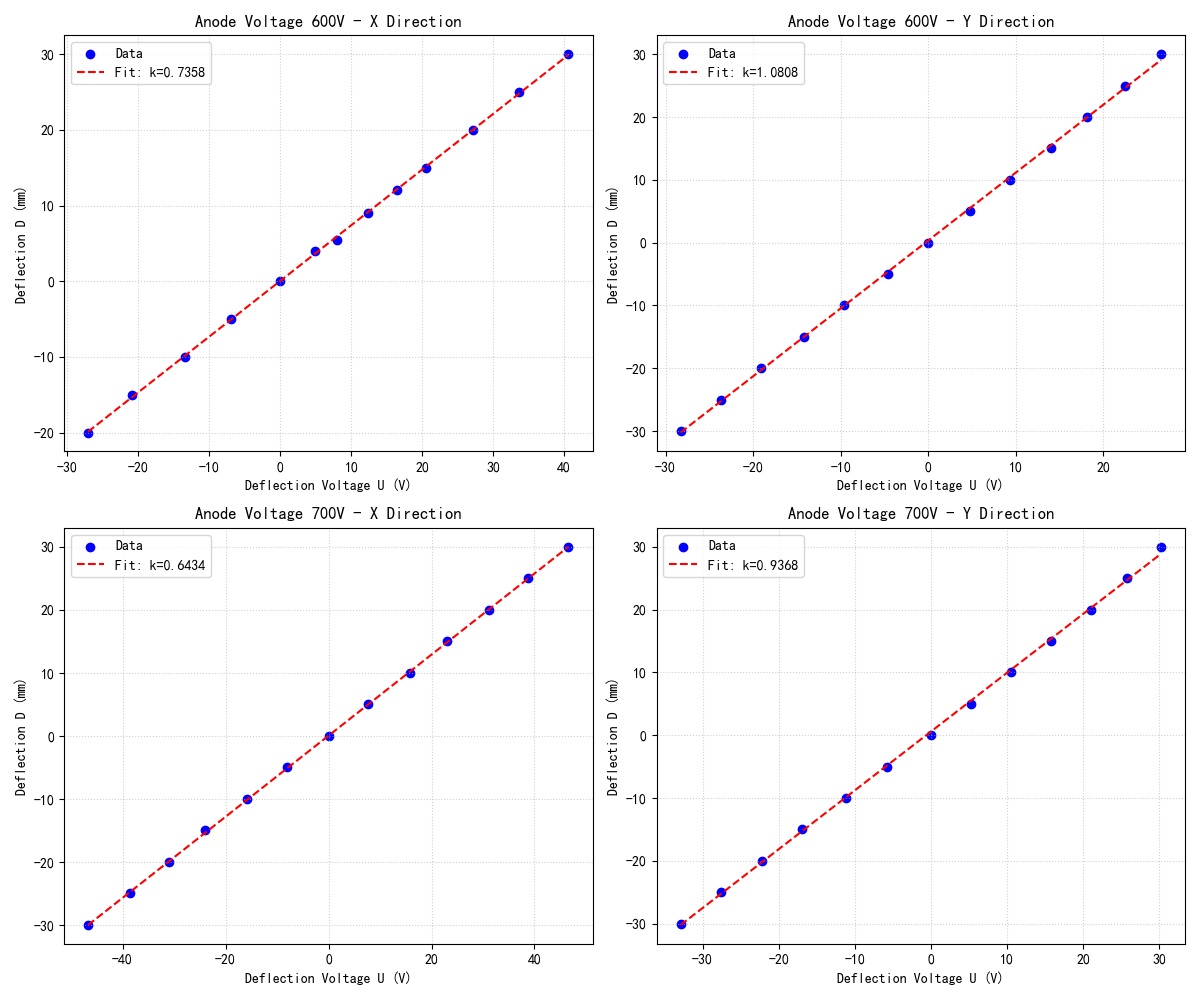
\includegraphics[width=0.9\textwidth]{deflection_plots.png}
    \caption{电子束电偏转 $U-D$ 关系曲线}
    \label{fig:deflection_plots}
\end{figure}

根据实验数据，通过线性拟合得到各条件下的电偏转灵敏度（即 $U-D$ 曲线斜率）如下：

\begin{itemize}
    \item 阳极电压 $U_2 = {600}{V}$ 时：
    \begin{itemize}
        \item X方向灵敏度 $S_x = {0.7358}{mm/V}$
        \item Y方向灵敏度 $S_y = {1.0808}{mm/V}$
    \end{itemize}
    \item 阳极电压 $U_2 = {700}{V}$ 时：
    \begin{itemize}
        \item X方向灵敏度 $S_x = {0.6434}{mm/V}$
        \item Y方向灵敏度 $S_y = {0.9368}{mm/V}$
    \end{itemize}
\end{itemize}
\subsection{磁偏转实验数据}
\begin{table}[H]
\centering
\caption{磁偏转灵敏度数据记录表}
\label{tab:mag_deflection}
\footnotesize
\setlength{\tabcolsep}{3pt}
\begin{tabular}{cccc}
\toprule
\multicolumn{2}{c}{阳极电压 $U_2 = 600$ V} & \multicolumn{2}{c}{阳极电压 $U_2 = 700$ V} \\
\cmidrule(lr){1-2} \cmidrule(lr){3-4}
$I$ (mA) & $D$ (mm) & $I$ (mA) & $D$ (mm) \\
\midrule
39   & 5   & 37   & 5   \\
79   & 10  & 77   & 10  \\
124  & 15  & 114  & 15  \\
167  & 20  & 155  & 20  \\
206  & 25  & 192  & 25  \\
245  & 30  & 228  & 30  \\
0    & 0.0 & 0    & 0.0 \\
-41  & -5  & -39  & -5  \\
-86  & -10 & -78  & -10 \\
-128 & -15 & -119 & -15 \\
-173 & -20 & -159 & -20 \\
-216 & -25 & -200 & -25 \\
-257 & -30 & -238 & -30 \\
\bottomrule
\end{tabular}
\end{table}

\begin{figure}[H]
    \centering
    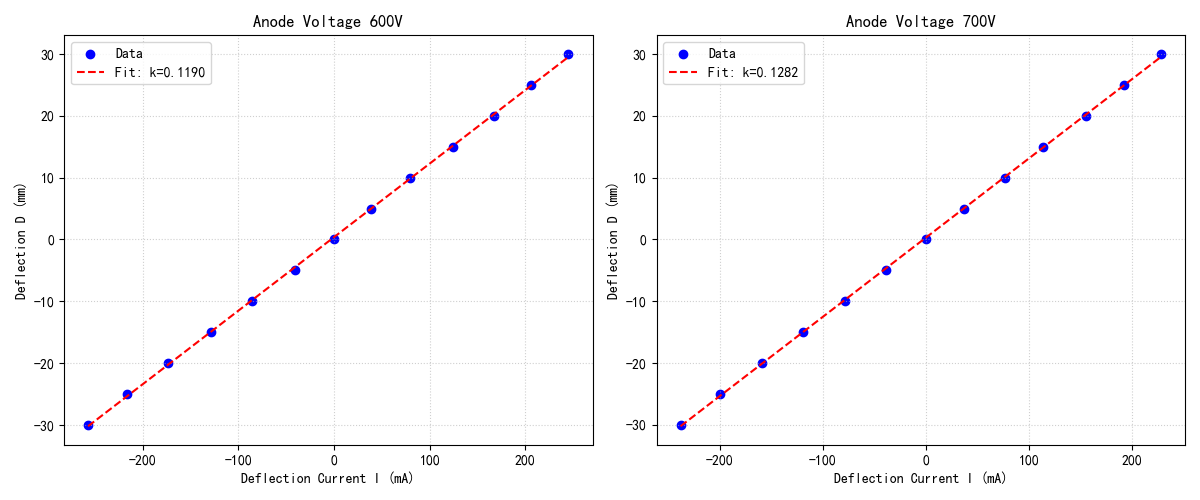
\includegraphics[width=0.9\textwidth]{magnetic_deflection_plots.png}
    \caption{电子束磁偏转 $I-D$ 关系曲线}
    \label{fig:mag_deflection_plots}
\end{figure}

根据实验数据，通过线性拟合得到各条件下的磁偏转灵敏度（即 $I-D$ 曲线斜率）如下：

\begin{itemize}
    \item 阳极电压 $U_2 = \SI{600}{V}$ 时：
    \begin{itemize}
        \item 磁偏转灵敏度 $S_m = \SI{0.1190}{mm/mA}$
    \end{itemize}
    \item 阳极电压 $U_2 = \SI{700}{V}$ 时：
    \begin{itemize}
        \item 磁偏转灵敏度 $S_m = \SI{0.1282}{mm/mA}$
    \end{itemize}
\end{itemize}

\subsection{电聚焦实验数据}
\begin{table}[H]
\centering
\caption{电聚焦电压关系表}
\label{tab:elec_focusing}
\footnotesize
\setlength{\tabcolsep}{3pt}
\begin{tabular}{lccccccccc}
\toprule
阳极电压 $V_2$ (V) & 600 & 650 & 700 & 750 & 800 & 850 & 900 & 950 & 1000 \\
聚焦电压 $V_1$ (V) & 133 & 137 & 142 & 153 & 164 & 170 & 180 & 191 & 198 \\
聚焦比 $V_2/V_1$ & 4.51 & 4.74 & 4.93 & 4.90 & 4.88 & 5.00 & 5.00 & 4.97 & 5.05 \\
\bottomrule
\end{tabular}
\end{table}

\begin{figure}[H]
    \centering
    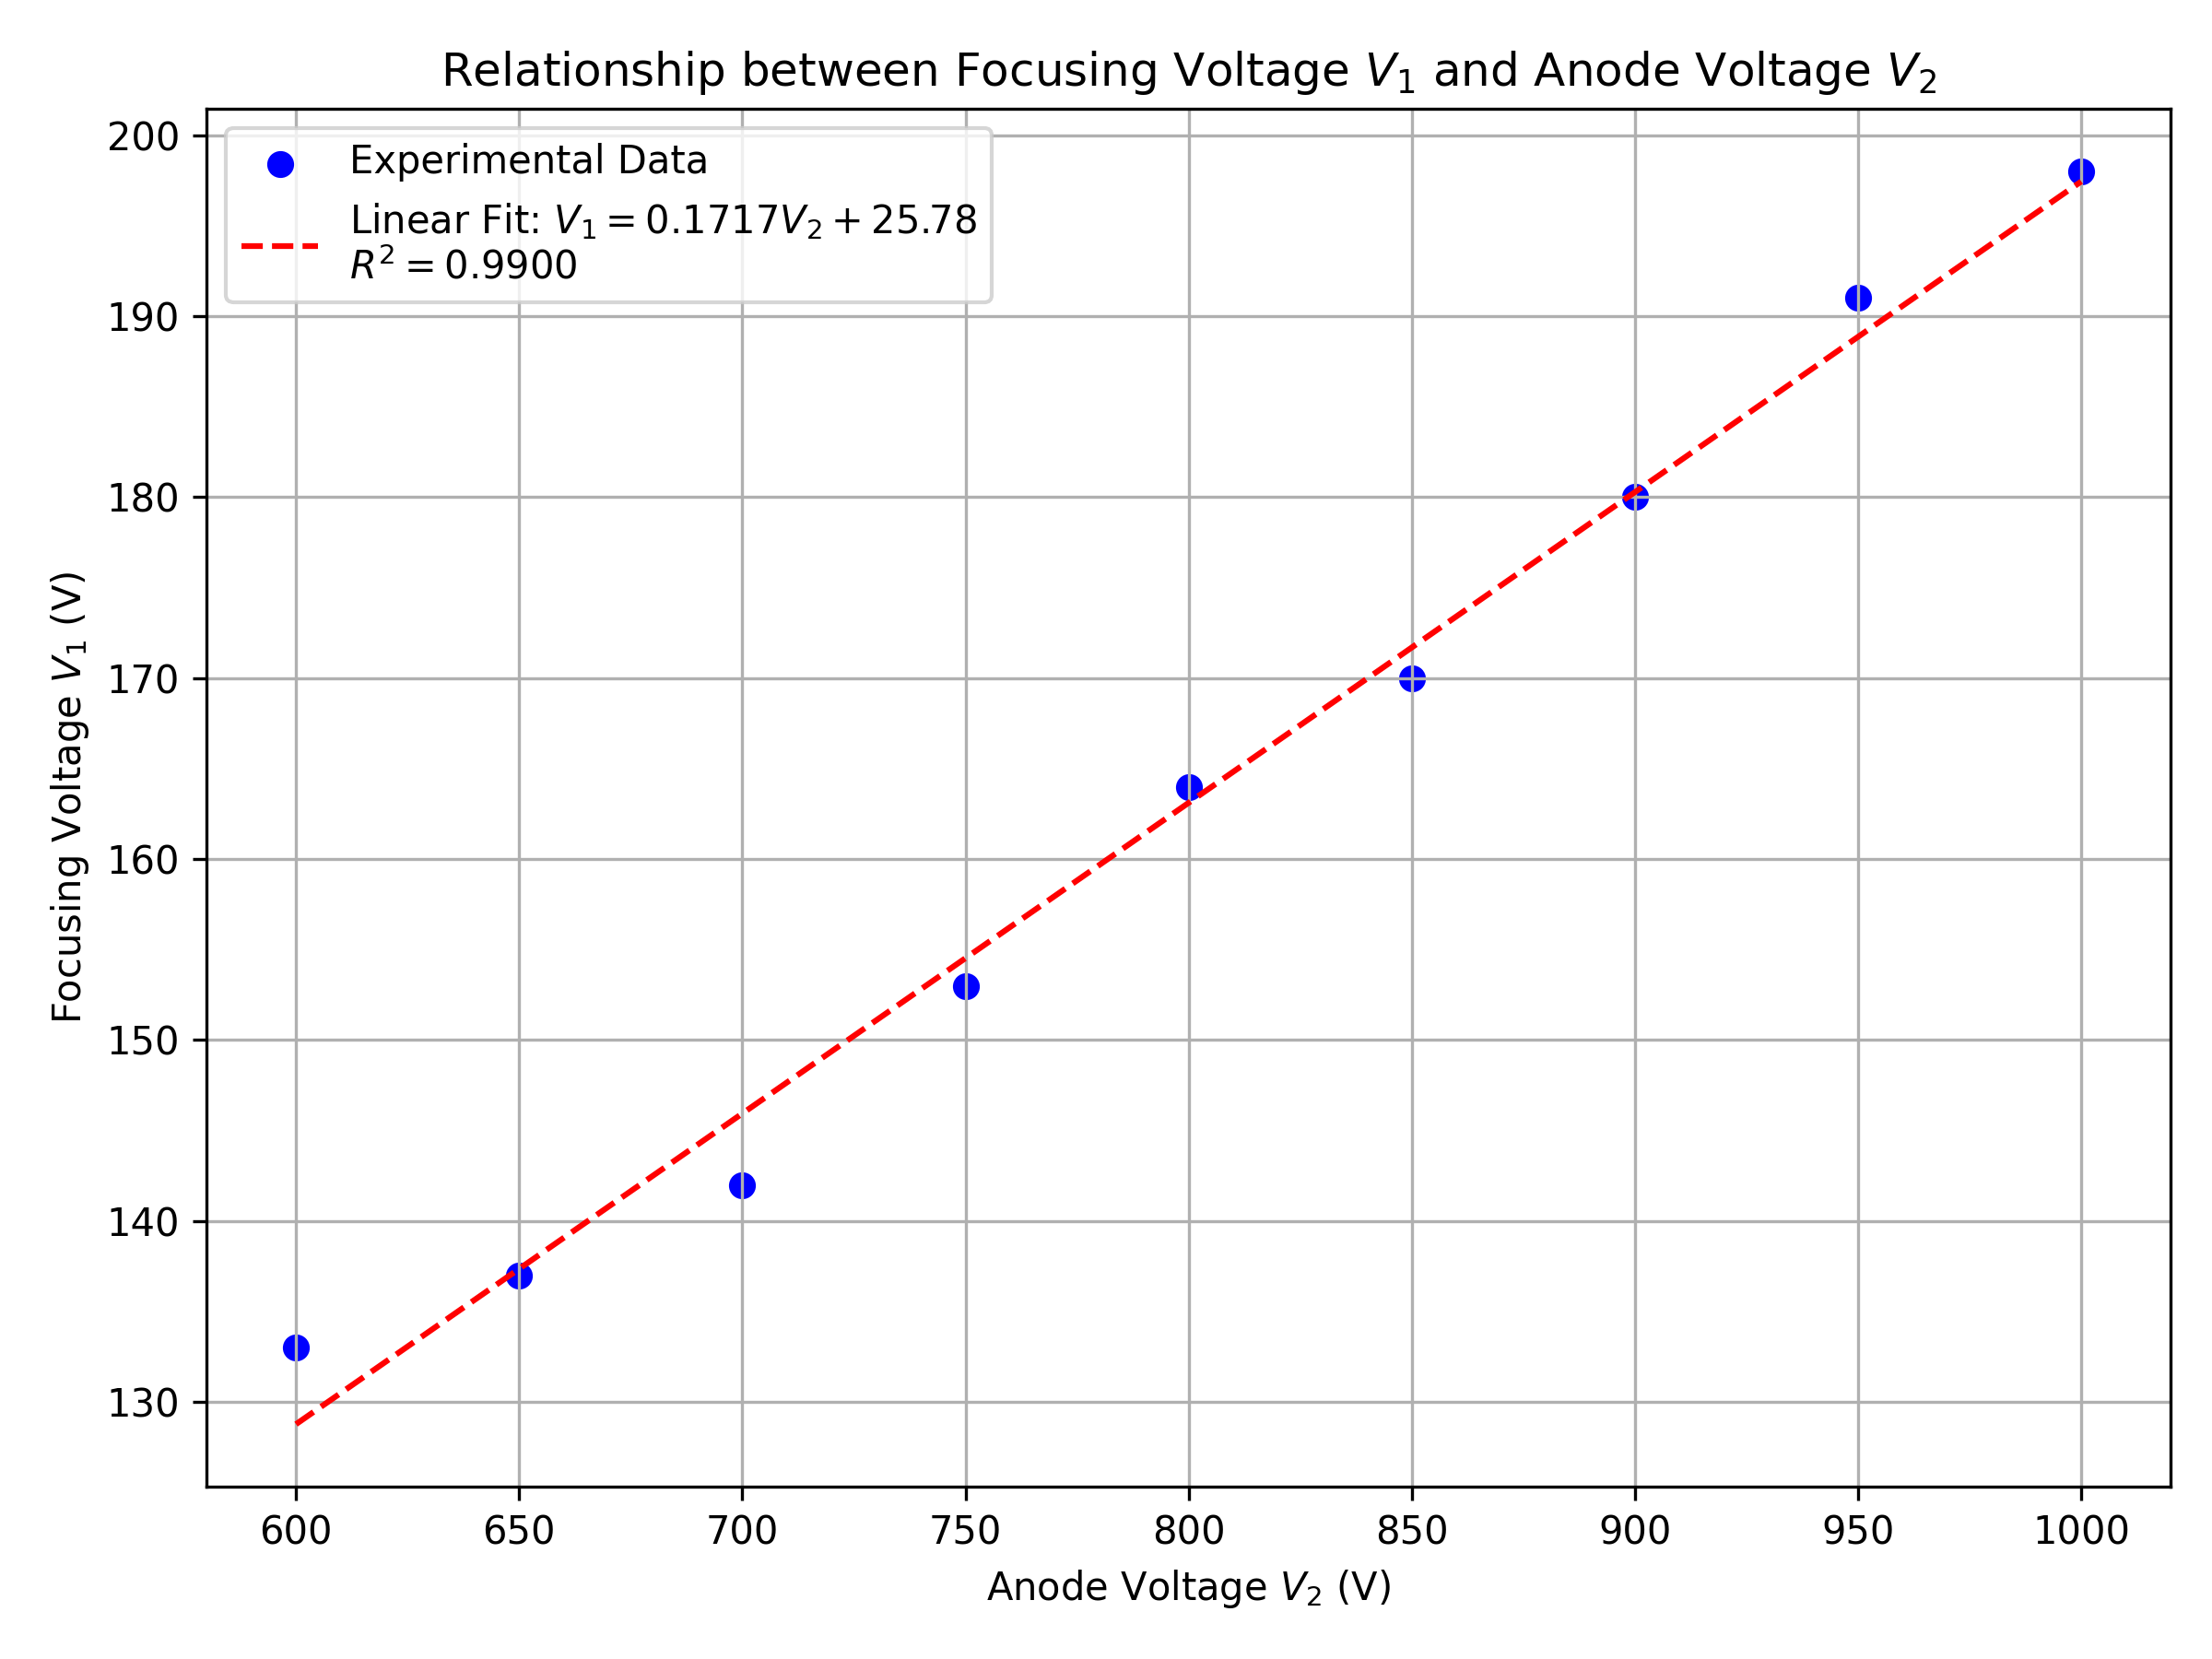
\includegraphics[width=0.7\textwidth]{focusing_plot.png}
    \caption{电聚焦电压 $V_1-V_2$ 关系曲线}
    \label{fig:focusing_plot}
\end{figure}

根据实验数据计算，不同阳极电压下的聚焦电压比值 $V_2/V_1$ 平均约为 4.89。通过线性回归分析，聚焦电压 $V_1$ 与阳极电压 $V_2$ 的拟合方程为 $V_1 = 0.1717 V_2 + 25.78$。相关系数 $r = 0.9950$，决定系数 $R^2 = 0.9900$，表明两者呈现高度显著的线性关系。
\subsection{电子荷质比实验数据}
\begin{table}[htbp]
\centering
\caption{电子荷质比测量数据}
\begin{tabular}{lcccc}
\toprule
\multirow{2}{*}{励磁电流} & \multicolumn{4}{c}{阳极电压} \\
\cmidrule(lr){2-5}
& 700V & 800V & 900V & 1000V \\
\midrule
$I_{\text{正}}$ (A) & 1.46 & 1.60 & 1.68 & 1.76 \\
$I_{\text{反}}$ (A) & 1.48 & 1.58 & 1.68 & 1.78 \\
$I_{\text{平均}}$ (A) & 1.47 & 1.59 & 1.68 & 1.77 \\
$e/m$ ($10^{11}$ C/kg) & 1.98 & 1.93 & 1.95 & 1.95 \\
\bottomrule
\end{tabular}
\end{table}

根据实验数据计算，不同阳极电压下的电子荷质比 $e/m$ 平均约为 $1.95 \times 10^{11} \mathrm{C/kg}$。与理论值 $e/m \approx 1.76 \times 10^{11} \mathrm{C/kg}$ 相比，相对误差约为 $10.9\%$。

\subsection{弗兰克赫兹手动测量数据记录表}
\begin{table}[htbp]
\centering
\caption{弗兰克-赫兹实验完整原始数据记录表（\textcolor{red}{红色}为波峰，\textcolor{blue}{蓝色}为波谷）}
\label{tab:fh_full_data}
\footnotesize
\setlength{\tabcolsep}{4pt}
\begin{tabular}{cccccccc}
\toprule
\multicolumn{2}{c}{\makebox[3.5cm]{第一列数据}} & \multicolumn{2}{c}{\makebox[3.5cm]{第二列数据}} & \multicolumn{2}{c}{\makebox[3.5cm]{第三列数据}} & \multicolumn{2}{c}{\makebox[3.5cm]{第四列数据}} \\
\cmidrule(lr){1-2} \cmidrule(lr){3-4} \cmidrule(lr){5-6} \cmidrule(lr){7-8}
$V_{G2K}$ (V) & $I_p$ ($\mu$A) & $V_{G2K}$ (V) & $I_p$ ($\mu$A) & $V_{G2K}$ (V) & $I_p$ ($\mu$A) & $V_{G2K}$ (V) & $I_p$ ($\mu$A) \\
\midrule
2.2 & 0.034 & 27.8 & 0.517 & 43.9 & 0.103 & 62.3 & 1.040 \\
5.4 & 0.033 & \textcolor{red}{28.0} & \textcolor{red}{0.519} & \textcolor{blue}{44.2} & \textcolor{blue}{0.092} & \textcolor{red}{62.6} & \textcolor{red}{1.042} \\
10.5 & 0.038 & 28.2 & 0.518 & 44.4 & 0.096 & 63.0 & 1.033 \\
12.5 & 0.091 & 28.4 & 0.517 & 44.4 & 0.100 & 63.0 & 1.005 \\
13.3 & 0.114 & 28.8 & 0.513 & 44.6 & 0.119 & 66.1 & 0.567 \\
14.2 & 0.144 & 29.1 & 0.500 & 45.0 & 0.151 & 67.1 & 0.350 \\
15.2 & 0.169 & 30.9 & 0.347 & 46.9 & 0.480 & \textcolor{blue}{67.7} & \textcolor{blue}{0.286} \\
16.2 & 0.197 & 31.5 & 0.267 & 48.1 & 0.709 & 68.2 & 0.296 \\
16.9 & 0.215 & 32.0 & 0.198 & 48.4 & 0.732 & 68.5 & 0.327 \\
17.4 & 0.227 & 32.4 & 0.154 & 49.0 & 0.808 & 71.7 & 0.841 \\
17.7 & 0.232 & 32.6 & 0.134 & 49.6 & 0.868 & 72.1 & 0.904 \\
18.1 & 0.239 & \textcolor{blue}{33.0} & \textcolor{blue}{0.112} & 50.0 & 0.877 & 72.6 & 0.976 \\
18.4 & 0.243 & 33.4 & 0.112 & 50.4 & 0.896 & 72.9 & 1.023 \\
18.6 & 0.245 & 33.6 & 0.123 & \textcolor{red}{51.0} & \textcolor{red}{0.900} & 73.3 & 1.077 \\
\textcolor{red}{18.8} & \textcolor{red}{0.248} & 34.0 & 0.157 & 51.5 & 0.875 & 73.7 & 1.114 \\
19.0 & 0.248 & 35.8 & 0.413 & 52.2 & 0.797 & 73.8 & 1.141 \\
19.2 & 0.246 & 36.2 & 0.470 & 52.9 & 0.684 & 74.4 & 1.156 \\
19.6 & 0.243 & 37.0 & 0.580 & 53.3 & 0.612 & 74.7 & 1.167 \\
19.8 & 0.237 & 37.4 & 0.604 & 54.1 & 0.434 & \textcolor{red}{75.1} & \textcolor{red}{1.169} \\
20.8 & 0.204 & 37.7 & 0.646 & 54.8 & 0.276 & 75.5 & 1.160 \\
21.1 & 0.192 & 38.0 & 0.671 & 55.2 & 0.191 & 79.0 & 0.629 \\
21.6 & 0.174 & 38.4 & 0.700 & 55.5 & 0.159 & 80.0 & 0.600 \\
21.8 & 0.166 & 38.5 & 0.694 & \textcolor{blue}{56.1} & \textcolor{blue}{0.158} & \textcolor{blue}{80.5} & \textcolor{blue}{0.520} \\
22.2 & 0.152 & 38.7 & 0.711 & 56.8 & 0.234 & 80.9 & 0.538 \\
\textcolor{blue}{22.5} & \textcolor{blue}{0.148} & 39.0 & 0.724 & 58.5 & 0.535 & 85.1 & 1.136 \\
22.8 & 0.153 & \textcolor{red}{39.5} & \textcolor{red}{0.727} & 59.1 & 0.637 & 85.5 & 1.194 \\
23.0 & 0.160 & 39.9 & 0.716 & 59.5 & 0.716 & 86.2 & 1.258 \\
23.7 & 0.202 & 40.1 & 0.704 & 60.0 & 0.809 & 87.1 & 1.323 \\
24.6 & 0.286 & 41.9 & 0.457 & 60.6 & 0.886 & 87.5 & 1.336 \\
25.6 & 0.384 & 42.6 & 0.326 & 61.0 & 0.941 & \textcolor{red}{88.0} & \textcolor{red}{1.337} \\
26.4 & 0.453 & 43.2 & 0.200 & 61.4 & 0.986 & 88.8 & 1.304 \\
27.1 & 0.487 & 43.6 & 0.134 & 61.9 & 1.019 &  &  \\
\bottomrule
\end{tabular}
\end{table}

\begin{figure}[H]
    \centering
    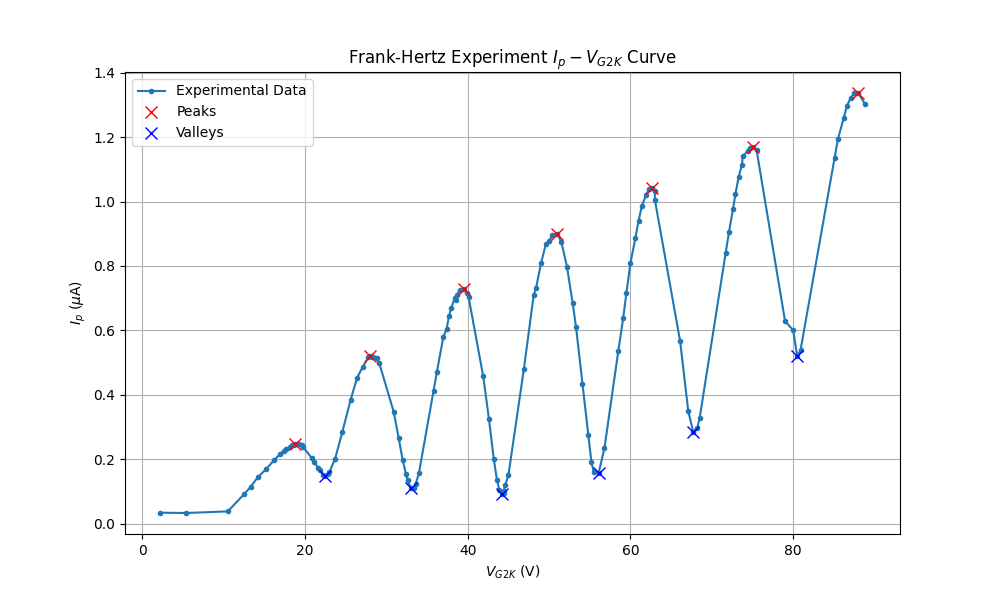
\includegraphics[width=0.9\textwidth]{fh_plot.png}
    \caption{弗兰克-赫兹实验 $I_p - V_{G2K}$ 曲线（含峰谷标注）}
    \label{fig:fh_plot}
\end{figure}

\begin{table}[htbp]
\centering
\caption{弗兰克-赫兹实验波峰与波谷位置记录表}
\label{tab:fh_peaks_valleys}
\begin{subtable}{\linewidth}
\centering
\caption{波峰位置数据}
\begin{tabular}{lccccccc}
\toprule
波峰序号 & 1 & 2 & 3 & 4 & 5 & 6 & 7 \\
\midrule
$V_{G2K}$ (V) & 18.8 & 28.0 & 39.5 & 51.0 & 62.6 & 75.1 & 88.0 \\
$I_p$ ($\mu$A) & 0.248 & 0.519 & 0.727 & 0.900 & 1.042 & 1.169 & 1.337 \\
\bottomrule
\end{tabular}
\end{subtable}

\vspace{1em}

\begin{subtable}{\linewidth}
\centering
\caption{波谷位置数据}
\begin{tabular}{lcccccc}
\toprule
波谷序号 & 1 & 2 & 3 & 4 & 5 & 6 \\
\midrule
$V_{G2K}$ (V) & 22.5 & 33.0 & 44.2 & 56.1 & 67.7 & 80.5 \\
$I_p$ ($\mu$A) & 0.148 & 0.112 & 0.092 & 0.158 & 0.286 & 0.520 \\
\bottomrule
\end{tabular}
\end{subtable}
\end{table}
观察图 \ref{fig:fh_plot} 所示的 $I_p - V_{G2K}$ 实验曲线，可以看出板极电流 $I_p$ 随加速电压 $V_{G2K}$ 的增加呈现出显著的周期性变化规律。曲线包含多个清晰的波峰和波谷，这直观地反映了电子与氩原子之间发生的能量交换过程。

当电子在加速场中获得的能量低于氩原子的第一激发电位时，电子与原子发生弹性碰撞，能量损失极小，电流随电压增加而增大。一旦电子能量达到第一激发电位，电子与原子发生非弹性碰撞，将大部分能量传递给原子使其激发，电子自身能量骤减，无法克服反向拒斥电场到达板极，导致电流急剧下降形成波谷。随着电压继续升高，电子再次被加速积累能量，电流重新上升，直至发生下一次非弹性碰撞。

此外，观察到随着 $V_{G2K}$ 的增大，各级波峰的电流幅值逐渐增大。这是由于加速电压提高后，阴极发射的电子束受空间电荷效应的限制减弱，且电子在管内的运动轨迹和散射情况使得更多电子能够到达板极。

根据表 \ref{tab:fh_peaks_valleys} 中的波峰和波谷数据，采用逐差法或线性回归法可计算原子的第一激发电位。为减小接触电位差及首个峰值可能存在的测量误差影响，此处采用线性回归法处理数据。

设峰/谷序号为 $n$，对应的电压为 $U_n$，建立线性关系 $U_n = n \cdot \Delta U + a$，其中斜率 $\Delta U$ 即为第一激发电位。

对波峰数据进行线性拟合：
\begin{equation}
    U_p = 11.60 n + 5.44 \quad (R^2 = 0.9981)
\end{equation}
得波峰间距平均值 $\Delta U_p = 11.60\,\mathrm{V}$。

对波谷数据进行线性拟合：
\begin{equation}
    U_v = 11.60 n + 10.07 \quad (R^2 = 0.9991)
\end{equation}
得波谷间距平均值 $\Delta U_v = 11.60\,\mathrm{V}$。

取两者的平均值作为测量结果：
\begin{equation}
    \overline{\Delta U} = \frac{\Delta U_p + \Delta U_v}{2} = 11.60\,\mathrm{V}
\end{equation}

根据实验讲义（2.1节仪器说明），本实验使用的是充氩弗兰克-赫兹管。氩原子的第一激发电位理论值为 $U_{theory} = 11.55\,\mathrm{V}$。
计算相对误差：
\begin{equation}
    E = \frac{|\overline{\Delta U} - U_{theory}|}{U_{theory}} \times 100\% = \frac{|11.60 - 11.55|}{11.55} \times 100\% \approx 0.45\%
\end{equation}

实验结果与氩原子的理论值吻合良好，验证了原子能级的存在及玻尔理论的正确性。


\subsection{弗兰克赫兹波形图测量数据}
\begin{figure}
    \centering
    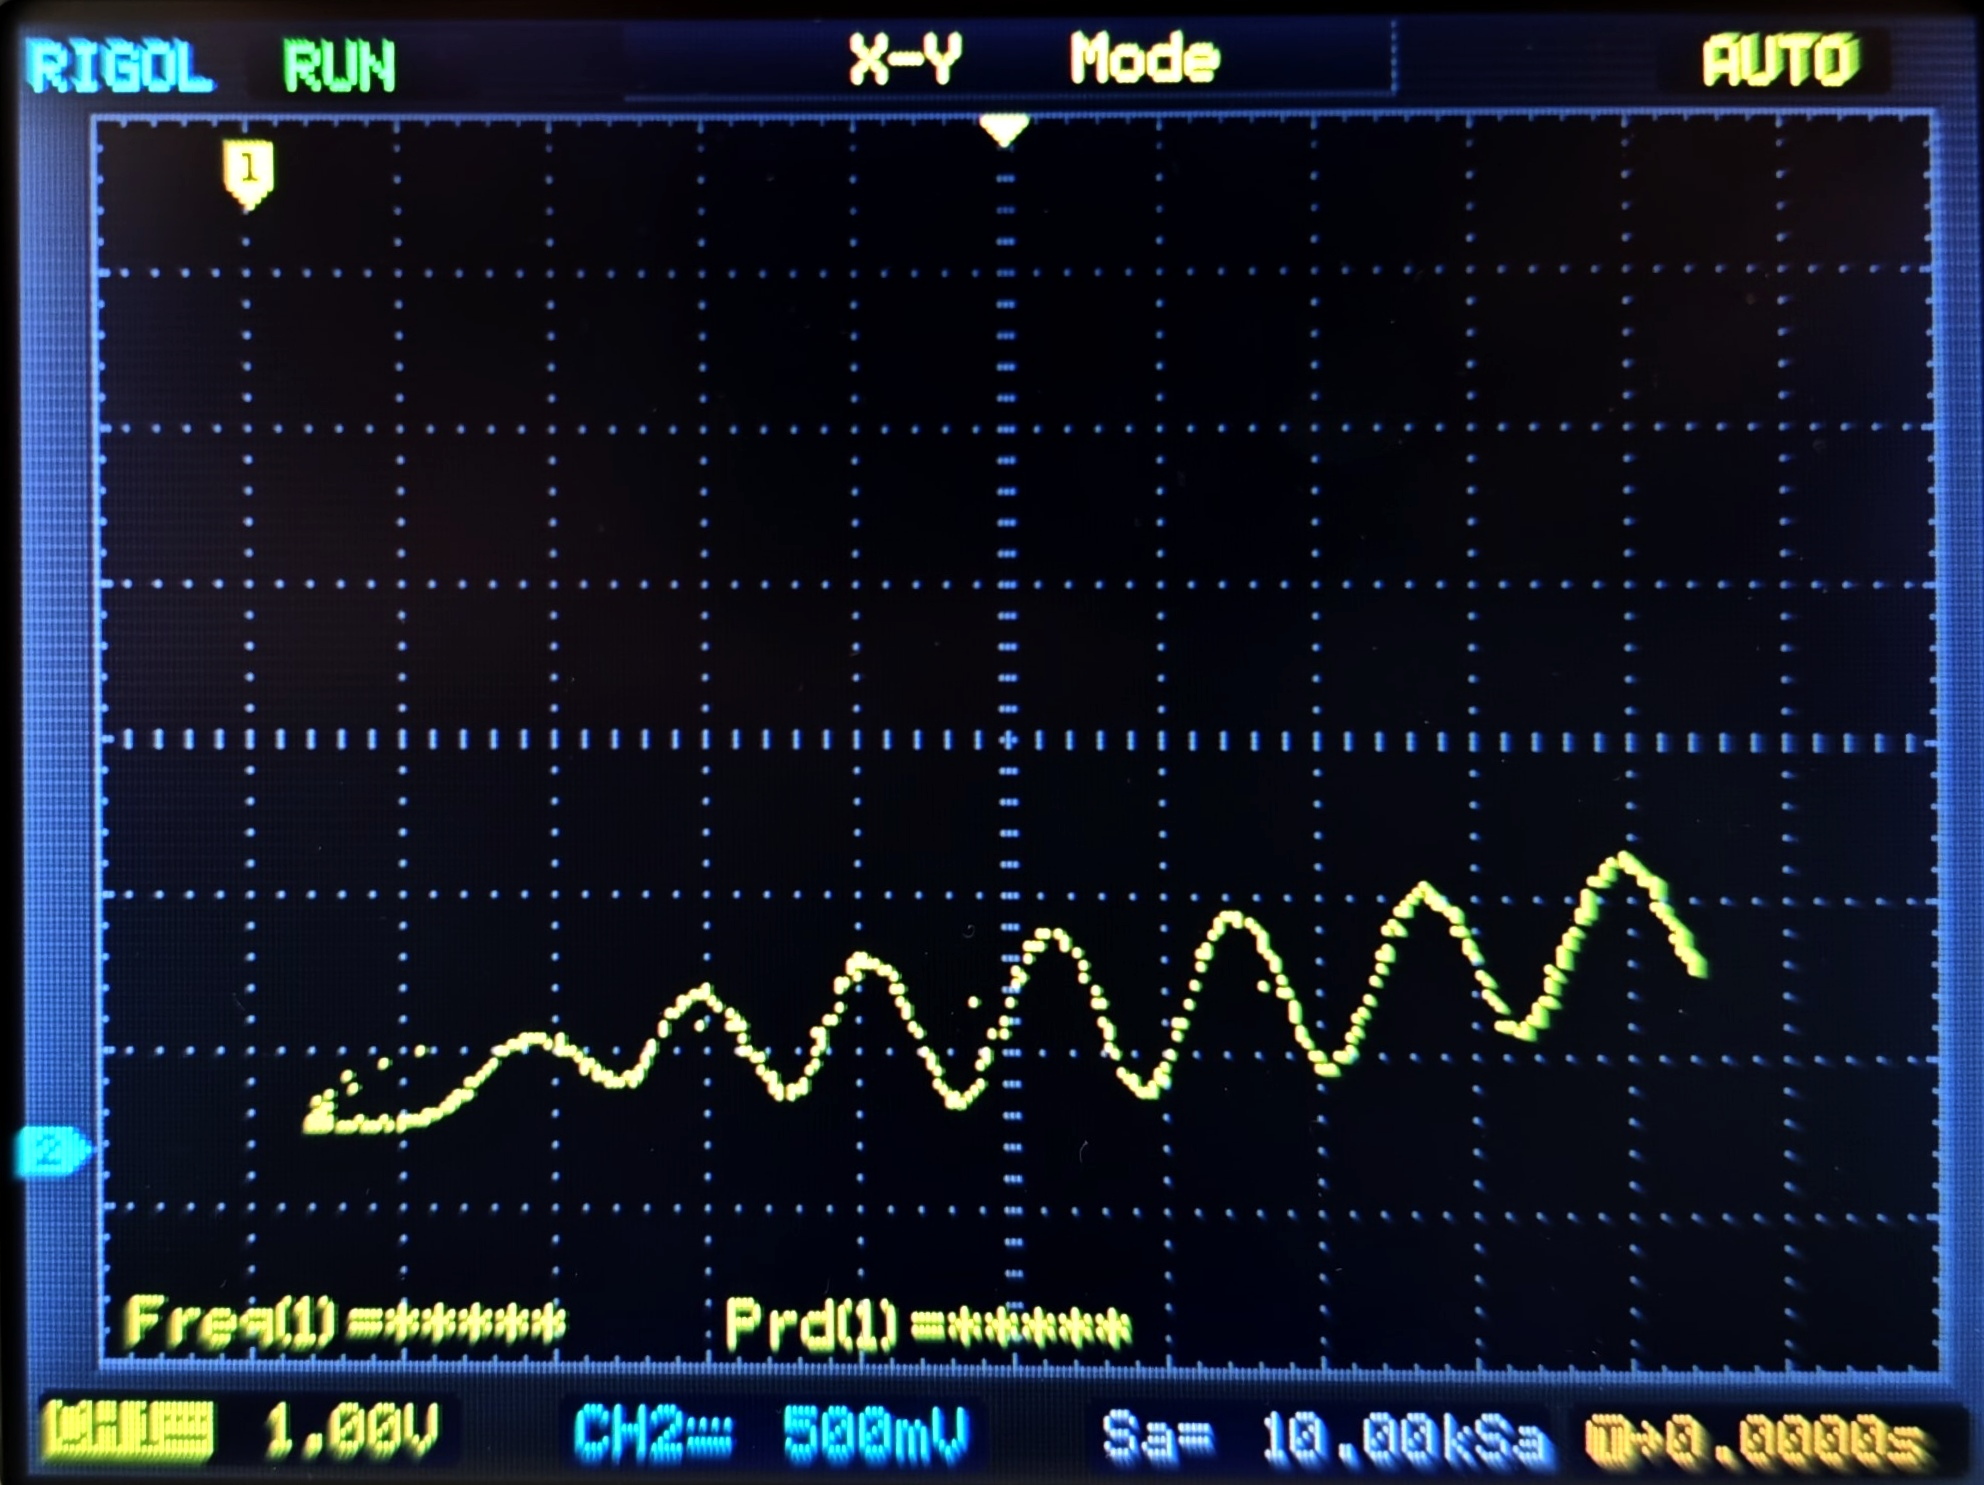
\includegraphics[width=0.9\textwidth]{fh_auto.jpg}
    \caption{弗兰克-赫兹实验示波器波形图}
    \label{fig:fh_auto}
    \end{figure}
图\ref{fig:fh_auto}为利用示波器 X-Y 模式观测到的弗兰克-赫兹实验扫描曲线。图中水平轴（CH1）对应栅极-阴极加速电压 $V_{G2K}$，垂直轴（CH2）对应到达板极的电流 $I_p$。

从波形图中可以清晰地观测到电流随电压变化呈现出显著的周期性“峰-谷”交替特征。这一现象直观地反映了电子与原子之间的能量交换过程：当电子在加速电场中获得的动能达到原子第一激发电位（或其整数倍）时，电子在栅极附近与原子发生非弹性碰撞，将能量传递给原子使其跃迁至激发态，而电子自身动能损失殆尽，无法克服反向拒斥电场到达板极，导致板极电流 $I_p$ 急剧下降形成波谷。当电压继续升高，电子再次被加速积累能量，电流重新上升直至下一次碰撞发生。

波形中相邻波峰（或波谷）在水平方向上的等间距分布，对应了原子的第一激发电位差值，验证了玻尔理论中关于原子能级不连续（量子化）的假设。此外，观察到随着加速电压的增加，各级波峰的电流幅值呈现逐渐递增的趋势，这主要归因于高电压下阴极电子发射效率的提高以及管内空间电荷效应的减弱，使得参与导电的有效电子数目增加。该实验图像信噪比良好，清晰地展示了至少 6 个完整的周期性振荡，有力地证实了原子内部存在分立的能级结构。

\section{思考题}

\begin{enumerate}
    \item \textbf{为什么最早的弗兰克-赫兹实验只能看见第一激发态的能级，该如何看到更高的能级？}
    
    \textbf{原因：} 
    在早期的弗兰克-赫兹实验中（通常使用汞蒸气），为了获得较大的极板电流，管内采用了较高的气体压强，使得气体原子密度较大，电子的平均自由程很短。
    由于电子与原子发生非弹性碰撞的概率（碰撞截面）非常大，电子在加速场中一旦获得相当于第一激发态的能量，就极有可能立刻与原子发生碰撞并将能量传递出去，导致电子很难积累足够的动能达到第二激发态或更高的能级。因此，实验中主要观察到的是基于第一激发电位的能量损失过程。
    
    \textbf{方法：} 
    若要观察到更高的能级，需要\textbf{降低管内的气体压强}（减小原子密度）。
    降低压强可以显著增大电子的平均自由程，使得电子在两次碰撞之间有更长的路程被电场加速，从而有机会在遇到原子之前积累到高于第一激发态的能量，进而激发原子的高能级状态。

    \item \textbf{弗兰克-赫兹实验中，波峰和波谷的间距受哪些参数影响？}
    
    波峰和波谷的间距 $\Delta U$ 主要受\textbf{气体原子的种类（原子内部能级结构）}决定，而与实验的电路参数（如灯丝电压、拒斥电压等）基本无关。
    
    \textbf{分析：}
    根据玻尔理论，波峰与波谷的间距对应于原子的第一激发电位 $U_0$，满足关系式 $e \Delta U = E_1 - E_0$。这是一个由原子自身性质决定的物理常数（例如氩气约为 11.5 eV，汞约为 4.9 eV）。
    \begin{itemize}
        \item \textbf{接触电位差}会影响整个曲线在电压轴上的左右平移（即影响第一个峰的位置），但不会改变后续峰之间的间距。
        \item \textbf{灯丝电压（温度）}会影响热电子的初速度分布，进而影响波形的清晰度和峰的宽度，但不会改变峰值的周期性间距。
    \end{itemize}
    因此，间距本质上只取决于充入实验管中的气体性质。
\end{enumerate}

\section{原始记录表和预习报告}
\begin{figure}[H]
    \centering
    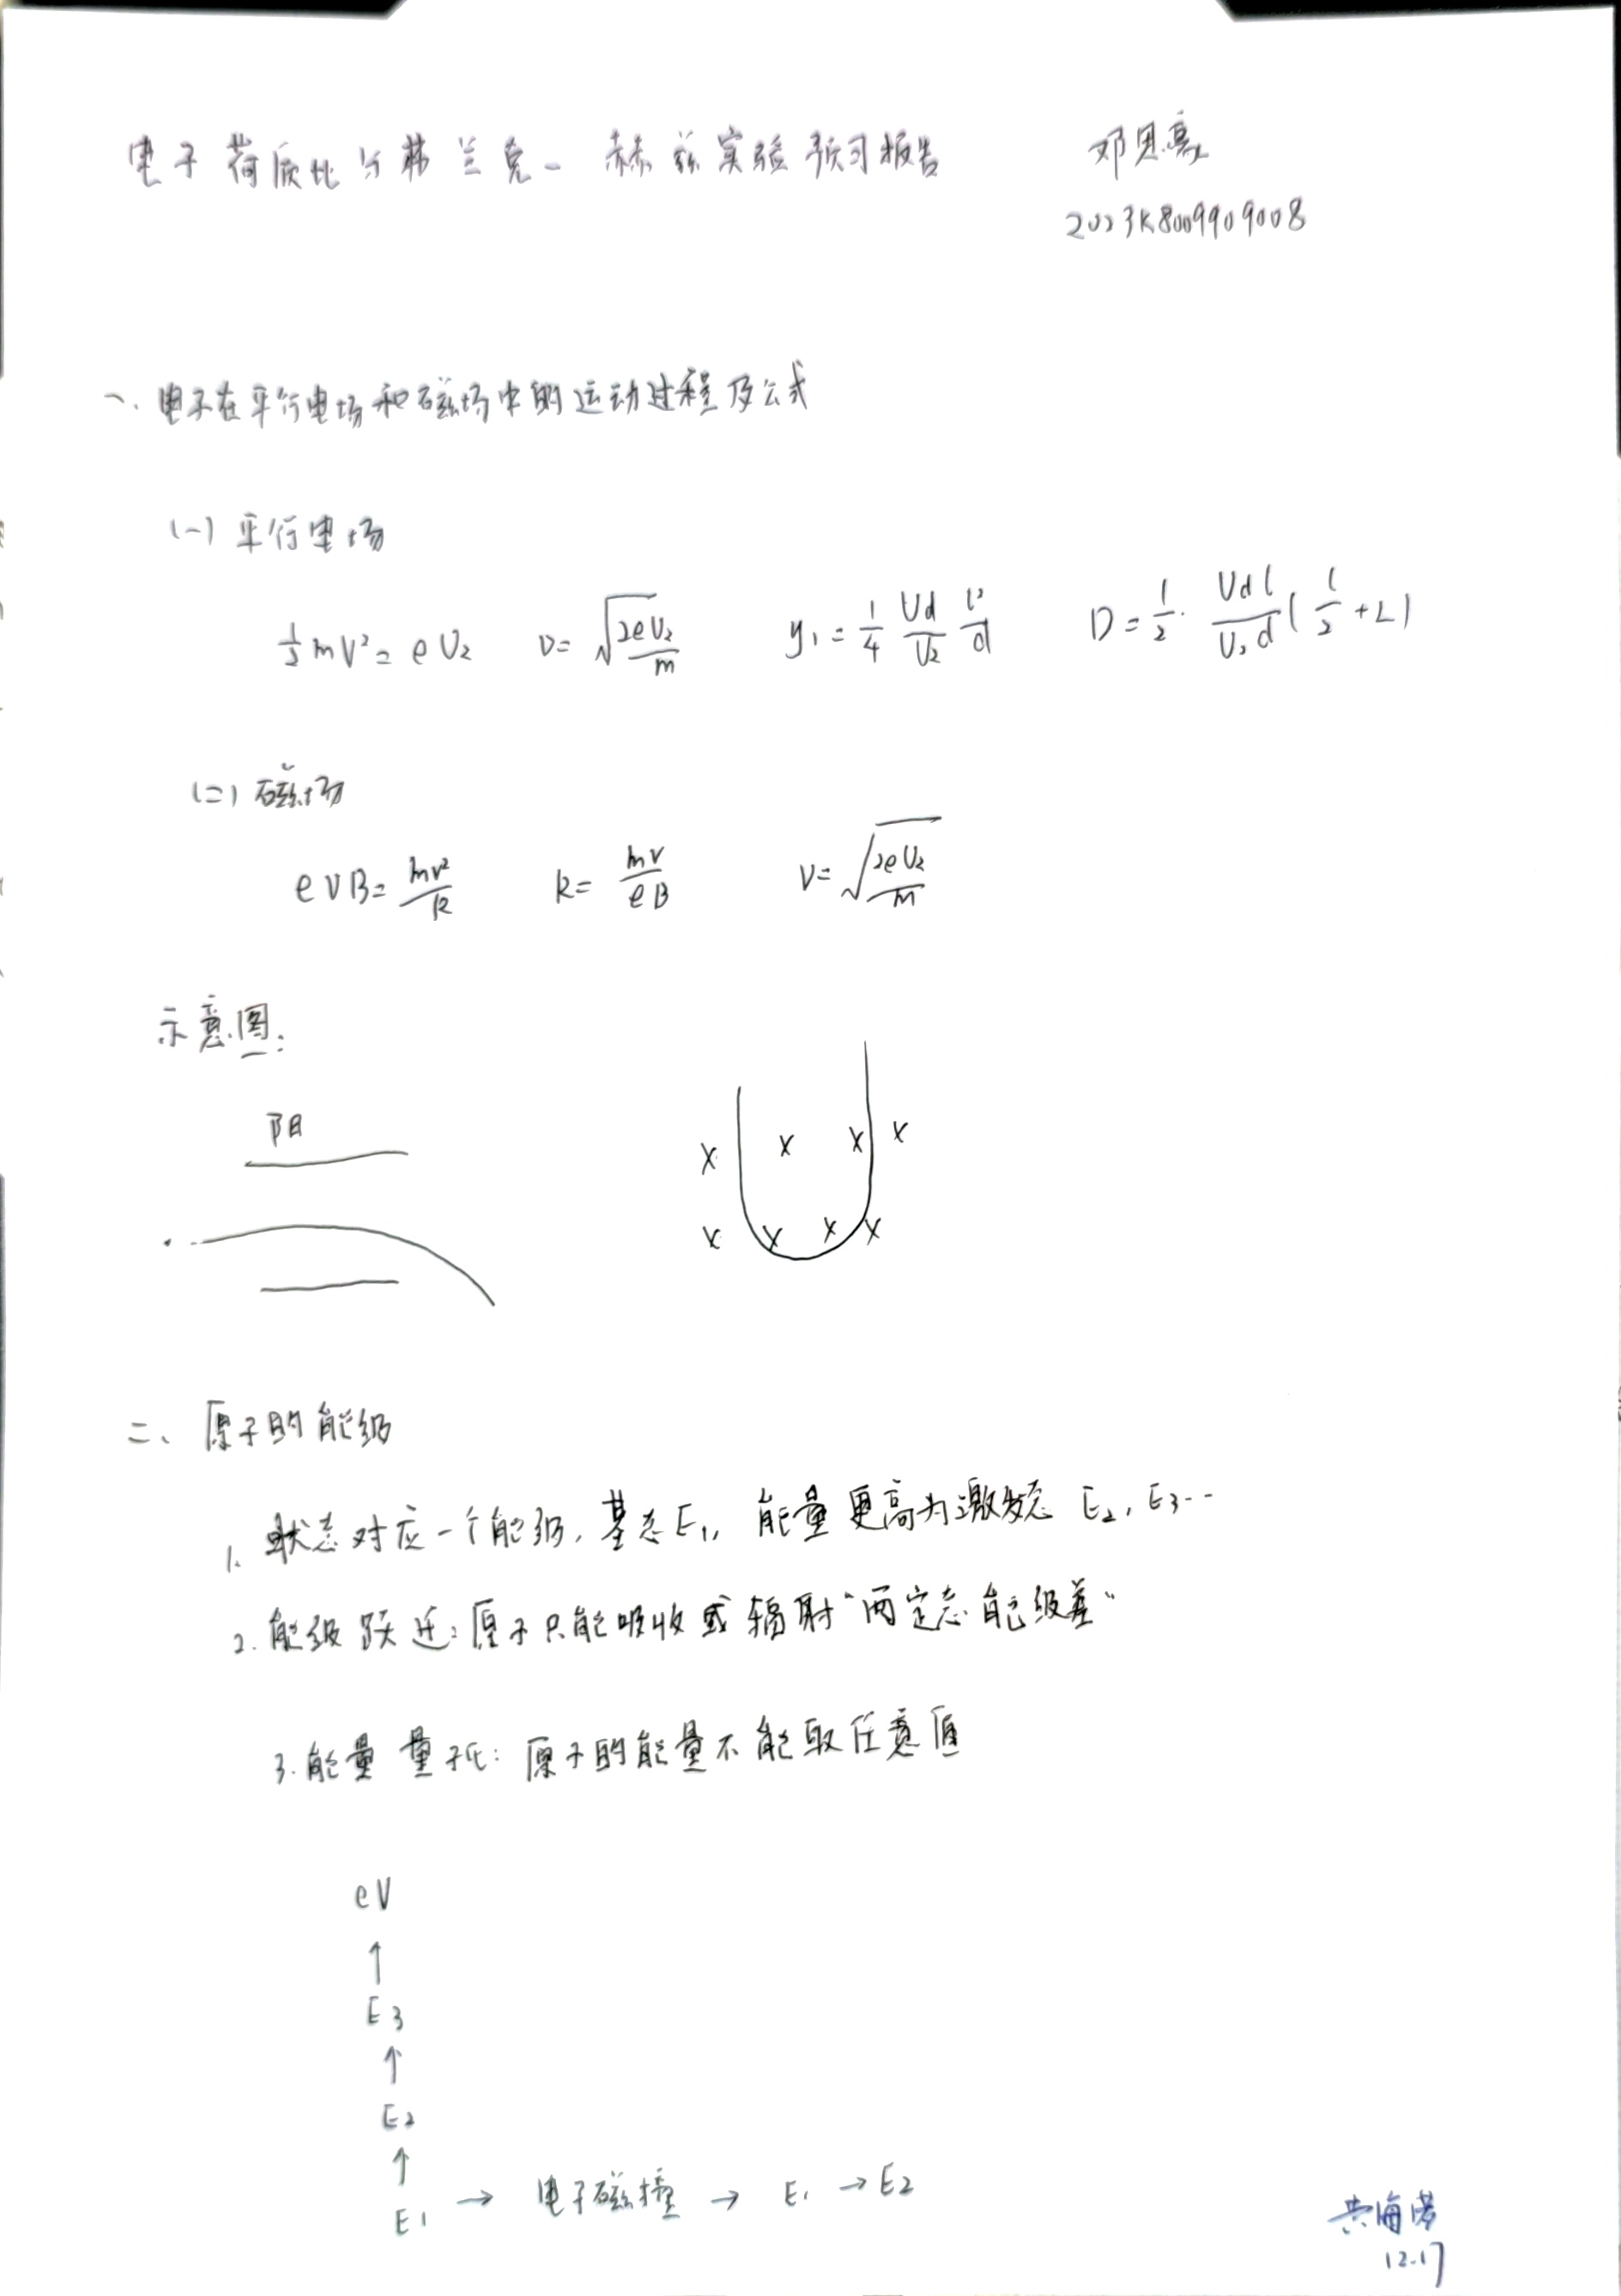
\includegraphics[width=0.9\textwidth]{report1.jpg}
    \caption{预习报告}
    \label{fig:original_record_1}
\end{figure}
\begin{figure}[H]
    \centering
    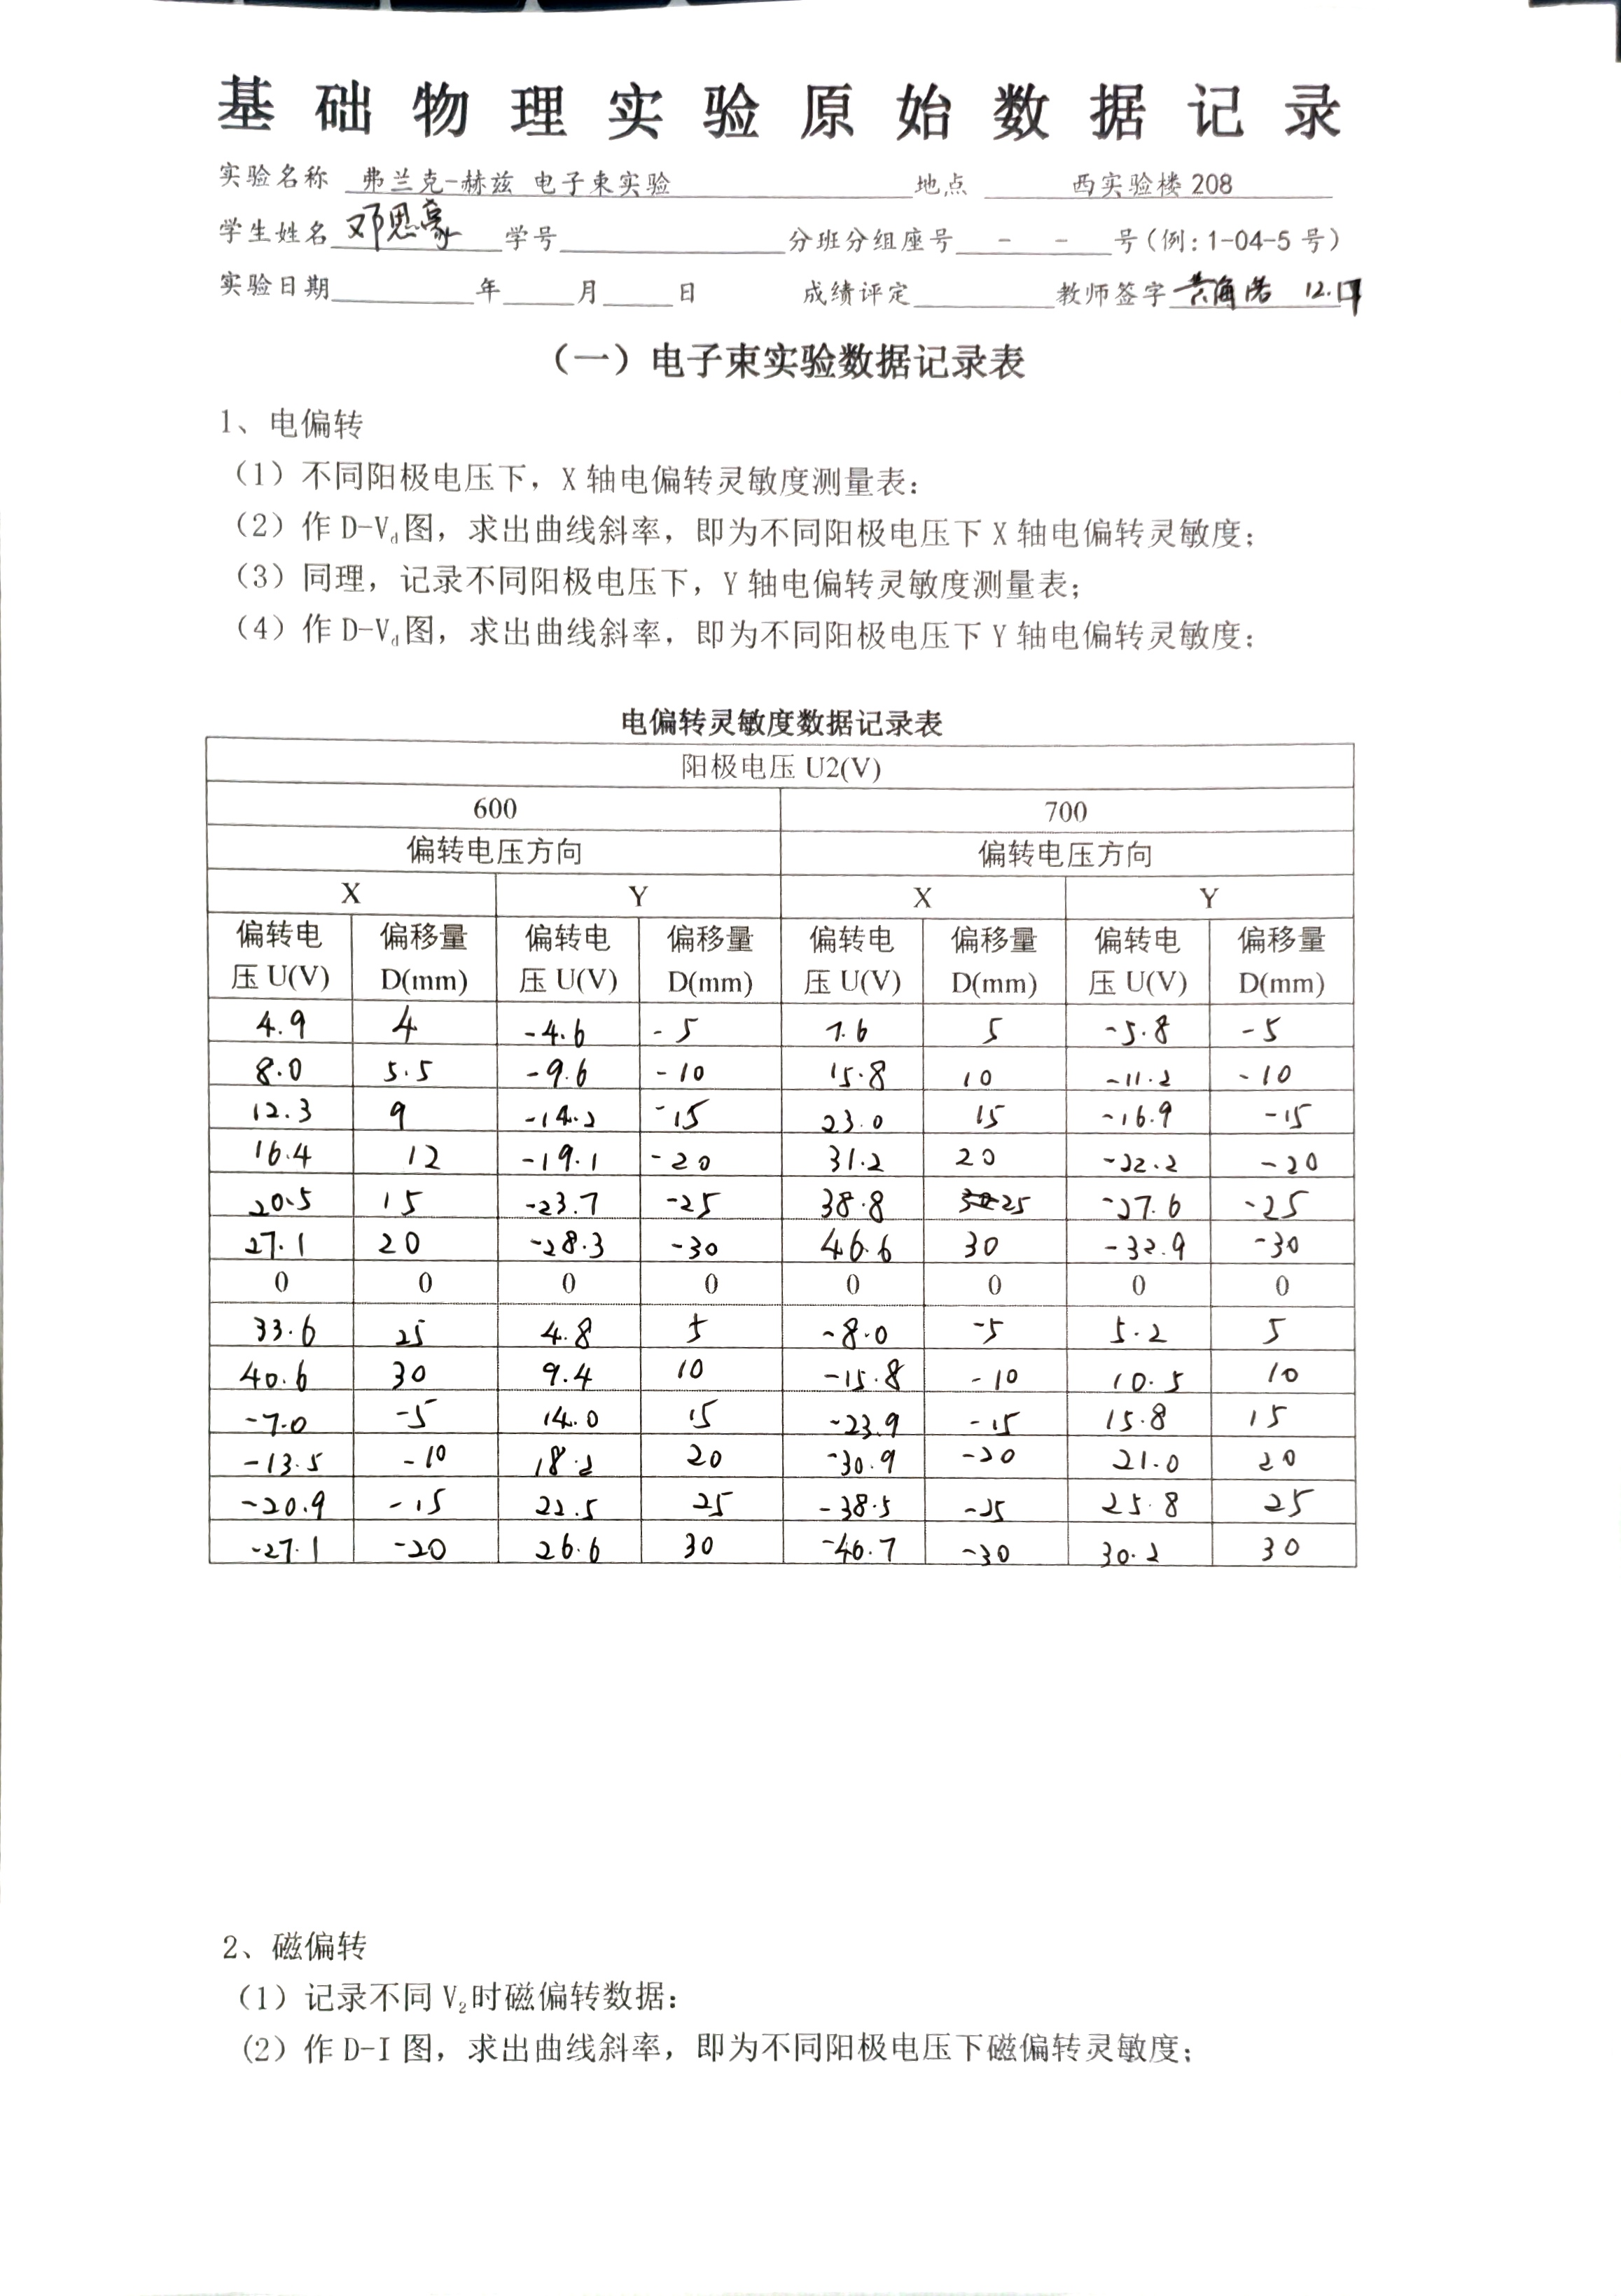
\includegraphics[width=0.9\textwidth]{report2.jpg}
    \caption{原始记录表页码1}
    \label{fig:original_record_2}
\end{figure}
\begin{figure}[H]
    \centering
    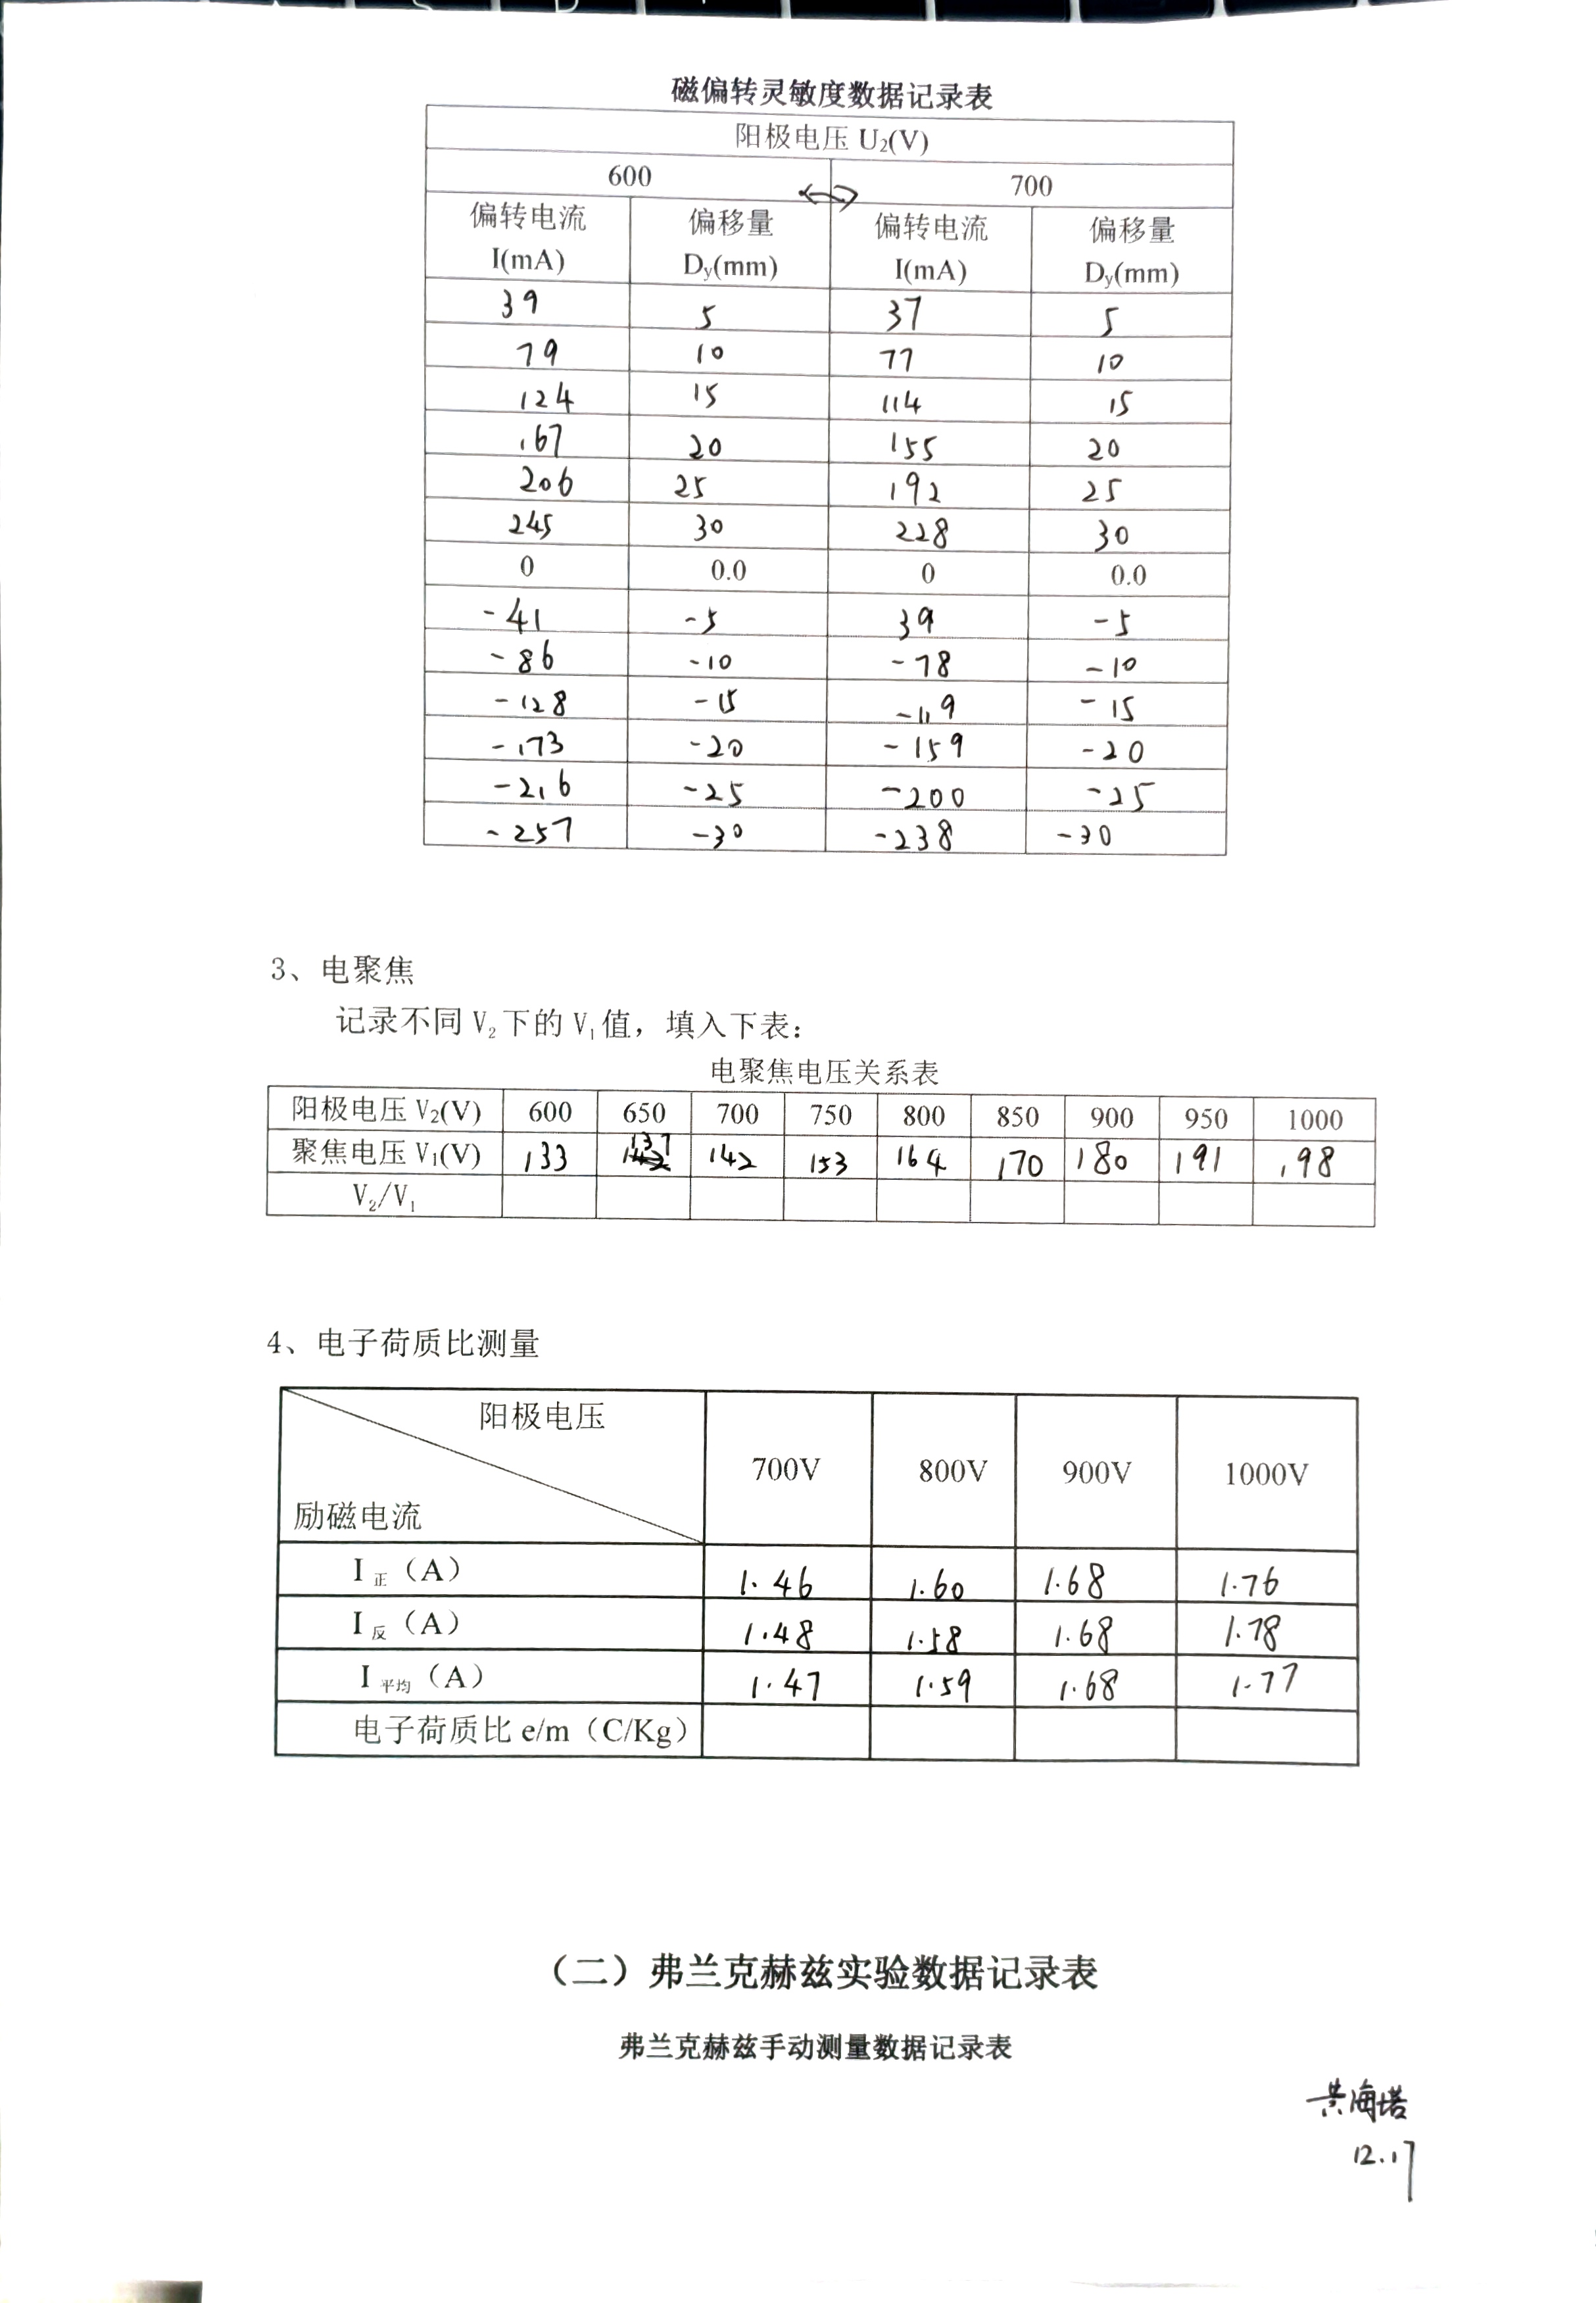
\includegraphics[width=0.9\textwidth]{report3.jpg}
    \caption{原始记录表页码2}
    \label{fig:original_record_3}
\end{figure}
\begin{figure}[H]
    \centering
    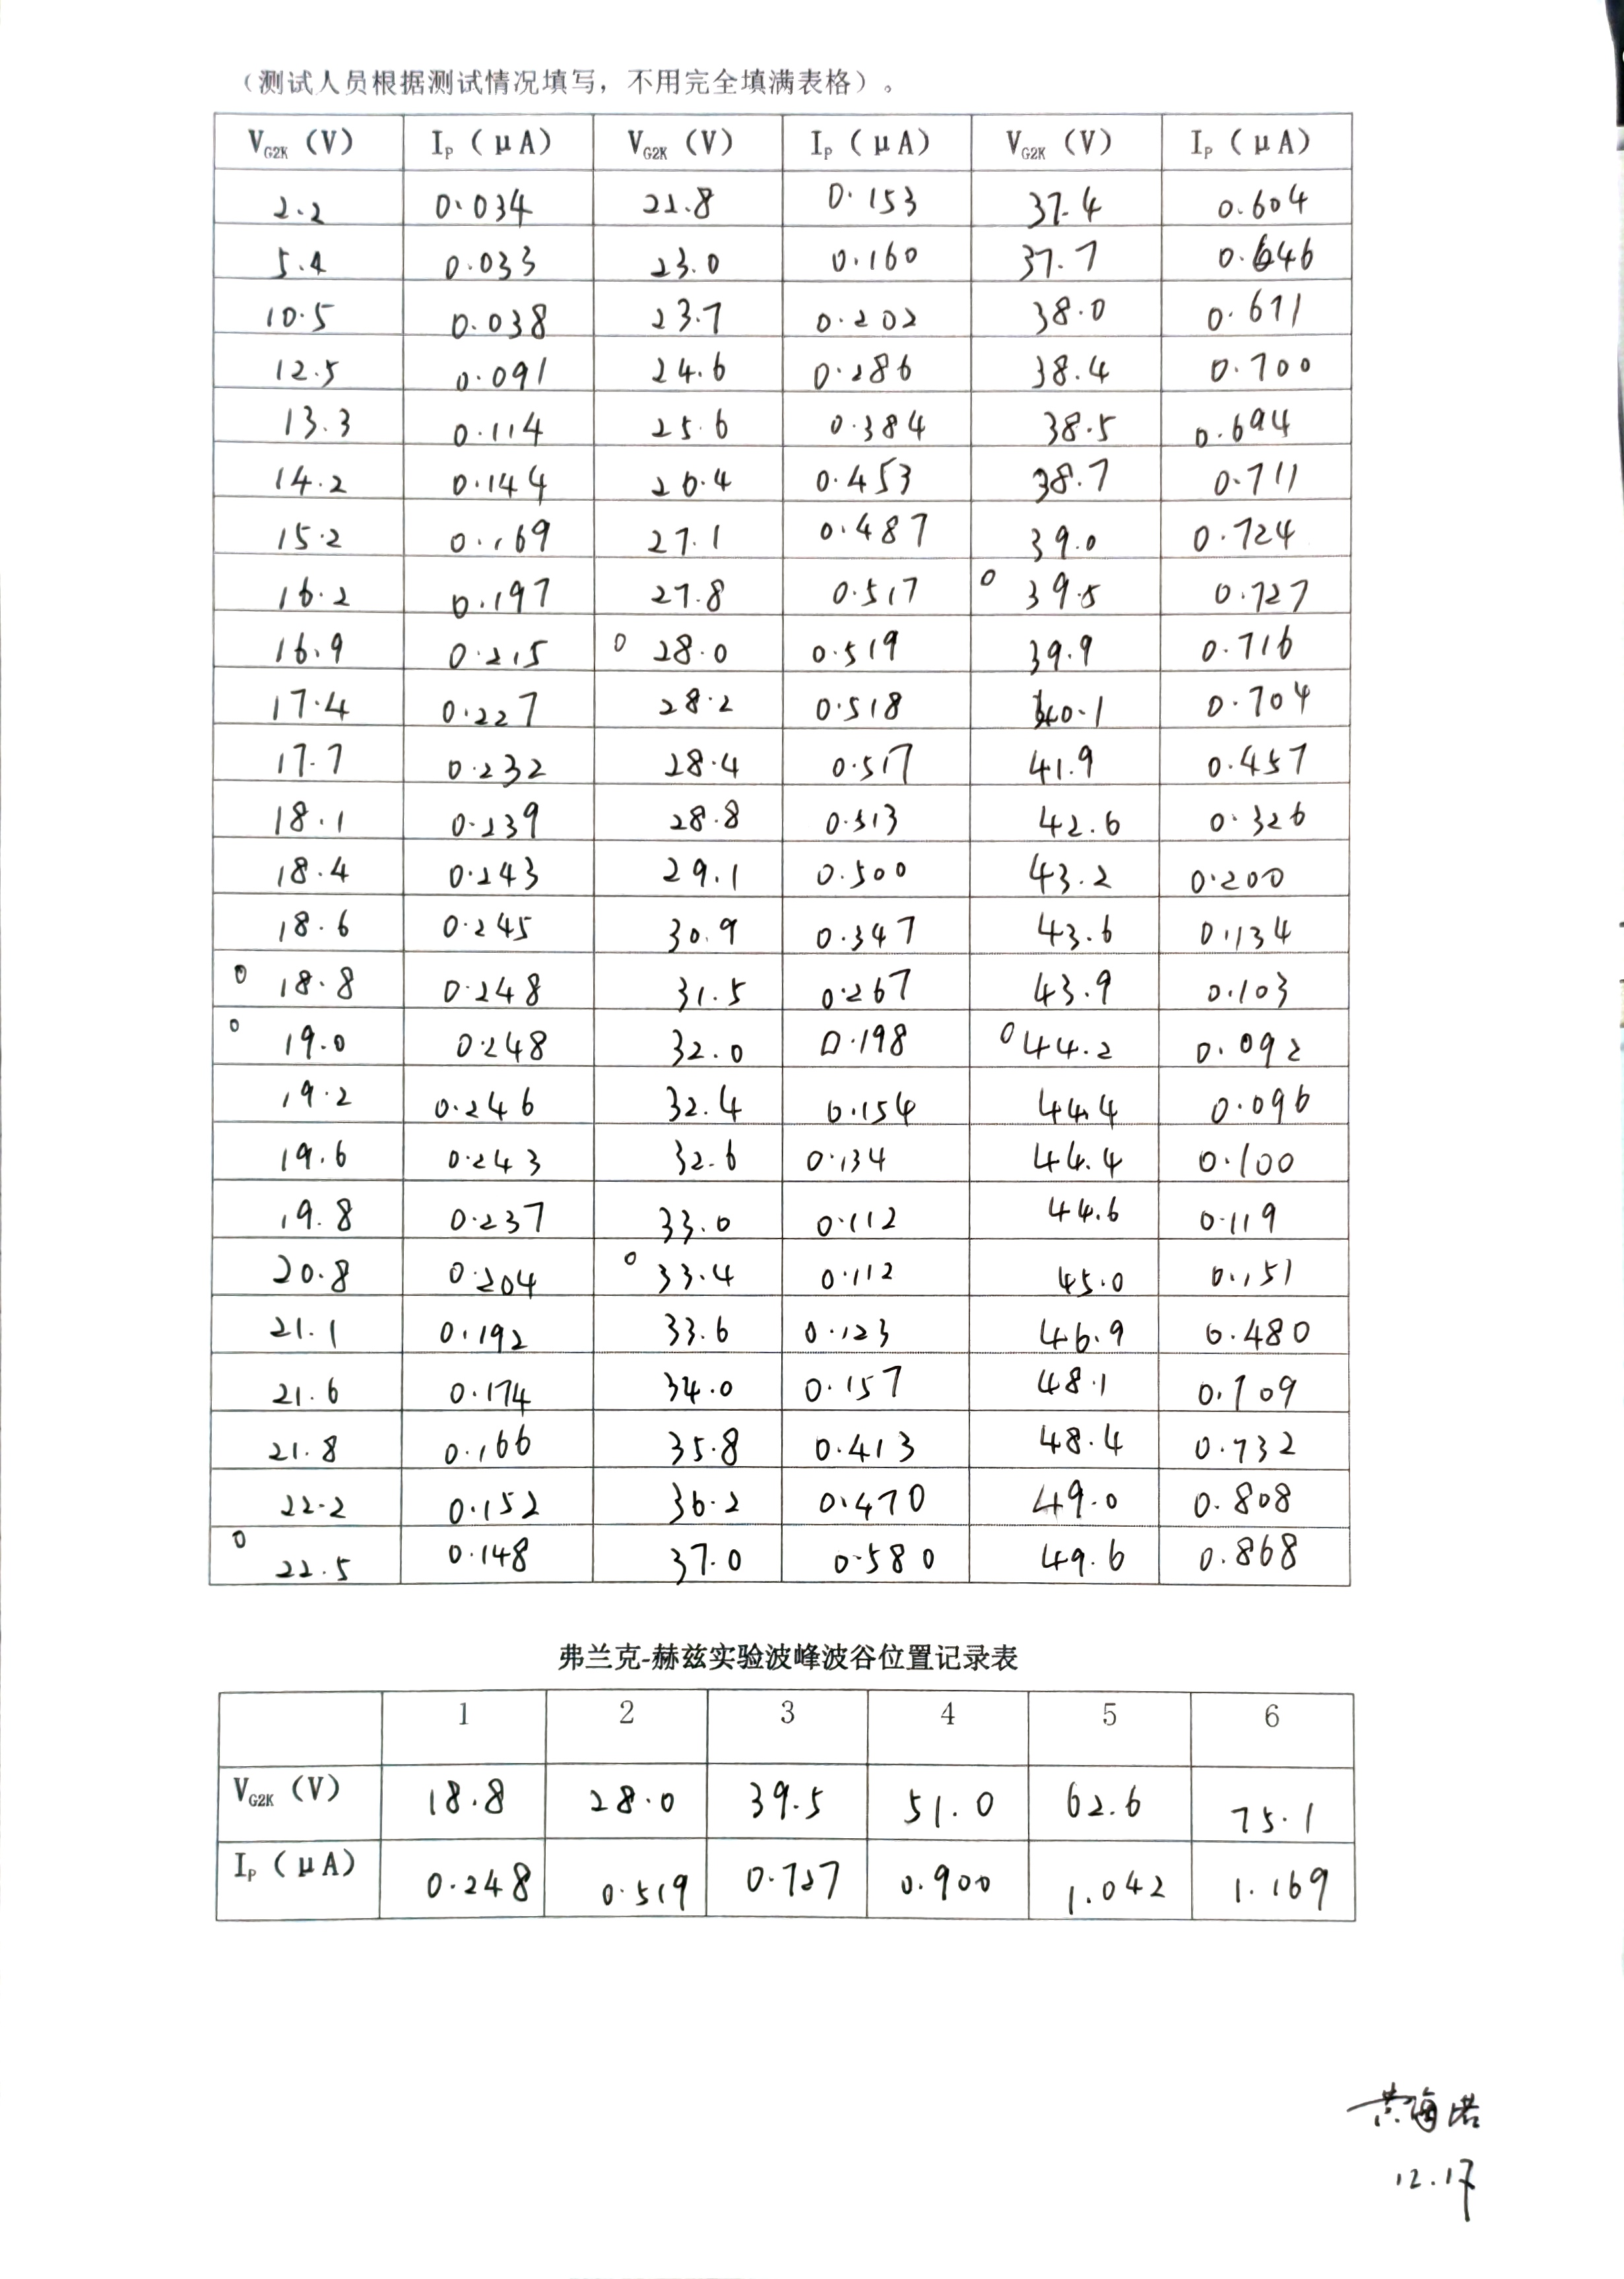
\includegraphics[width=0.9\textwidth]{report4.jpg}
    \caption{原始记录表页码3}
    \label{fig:original_record_4}
\end{figure}
\begin{figure}[H]
    \centering
    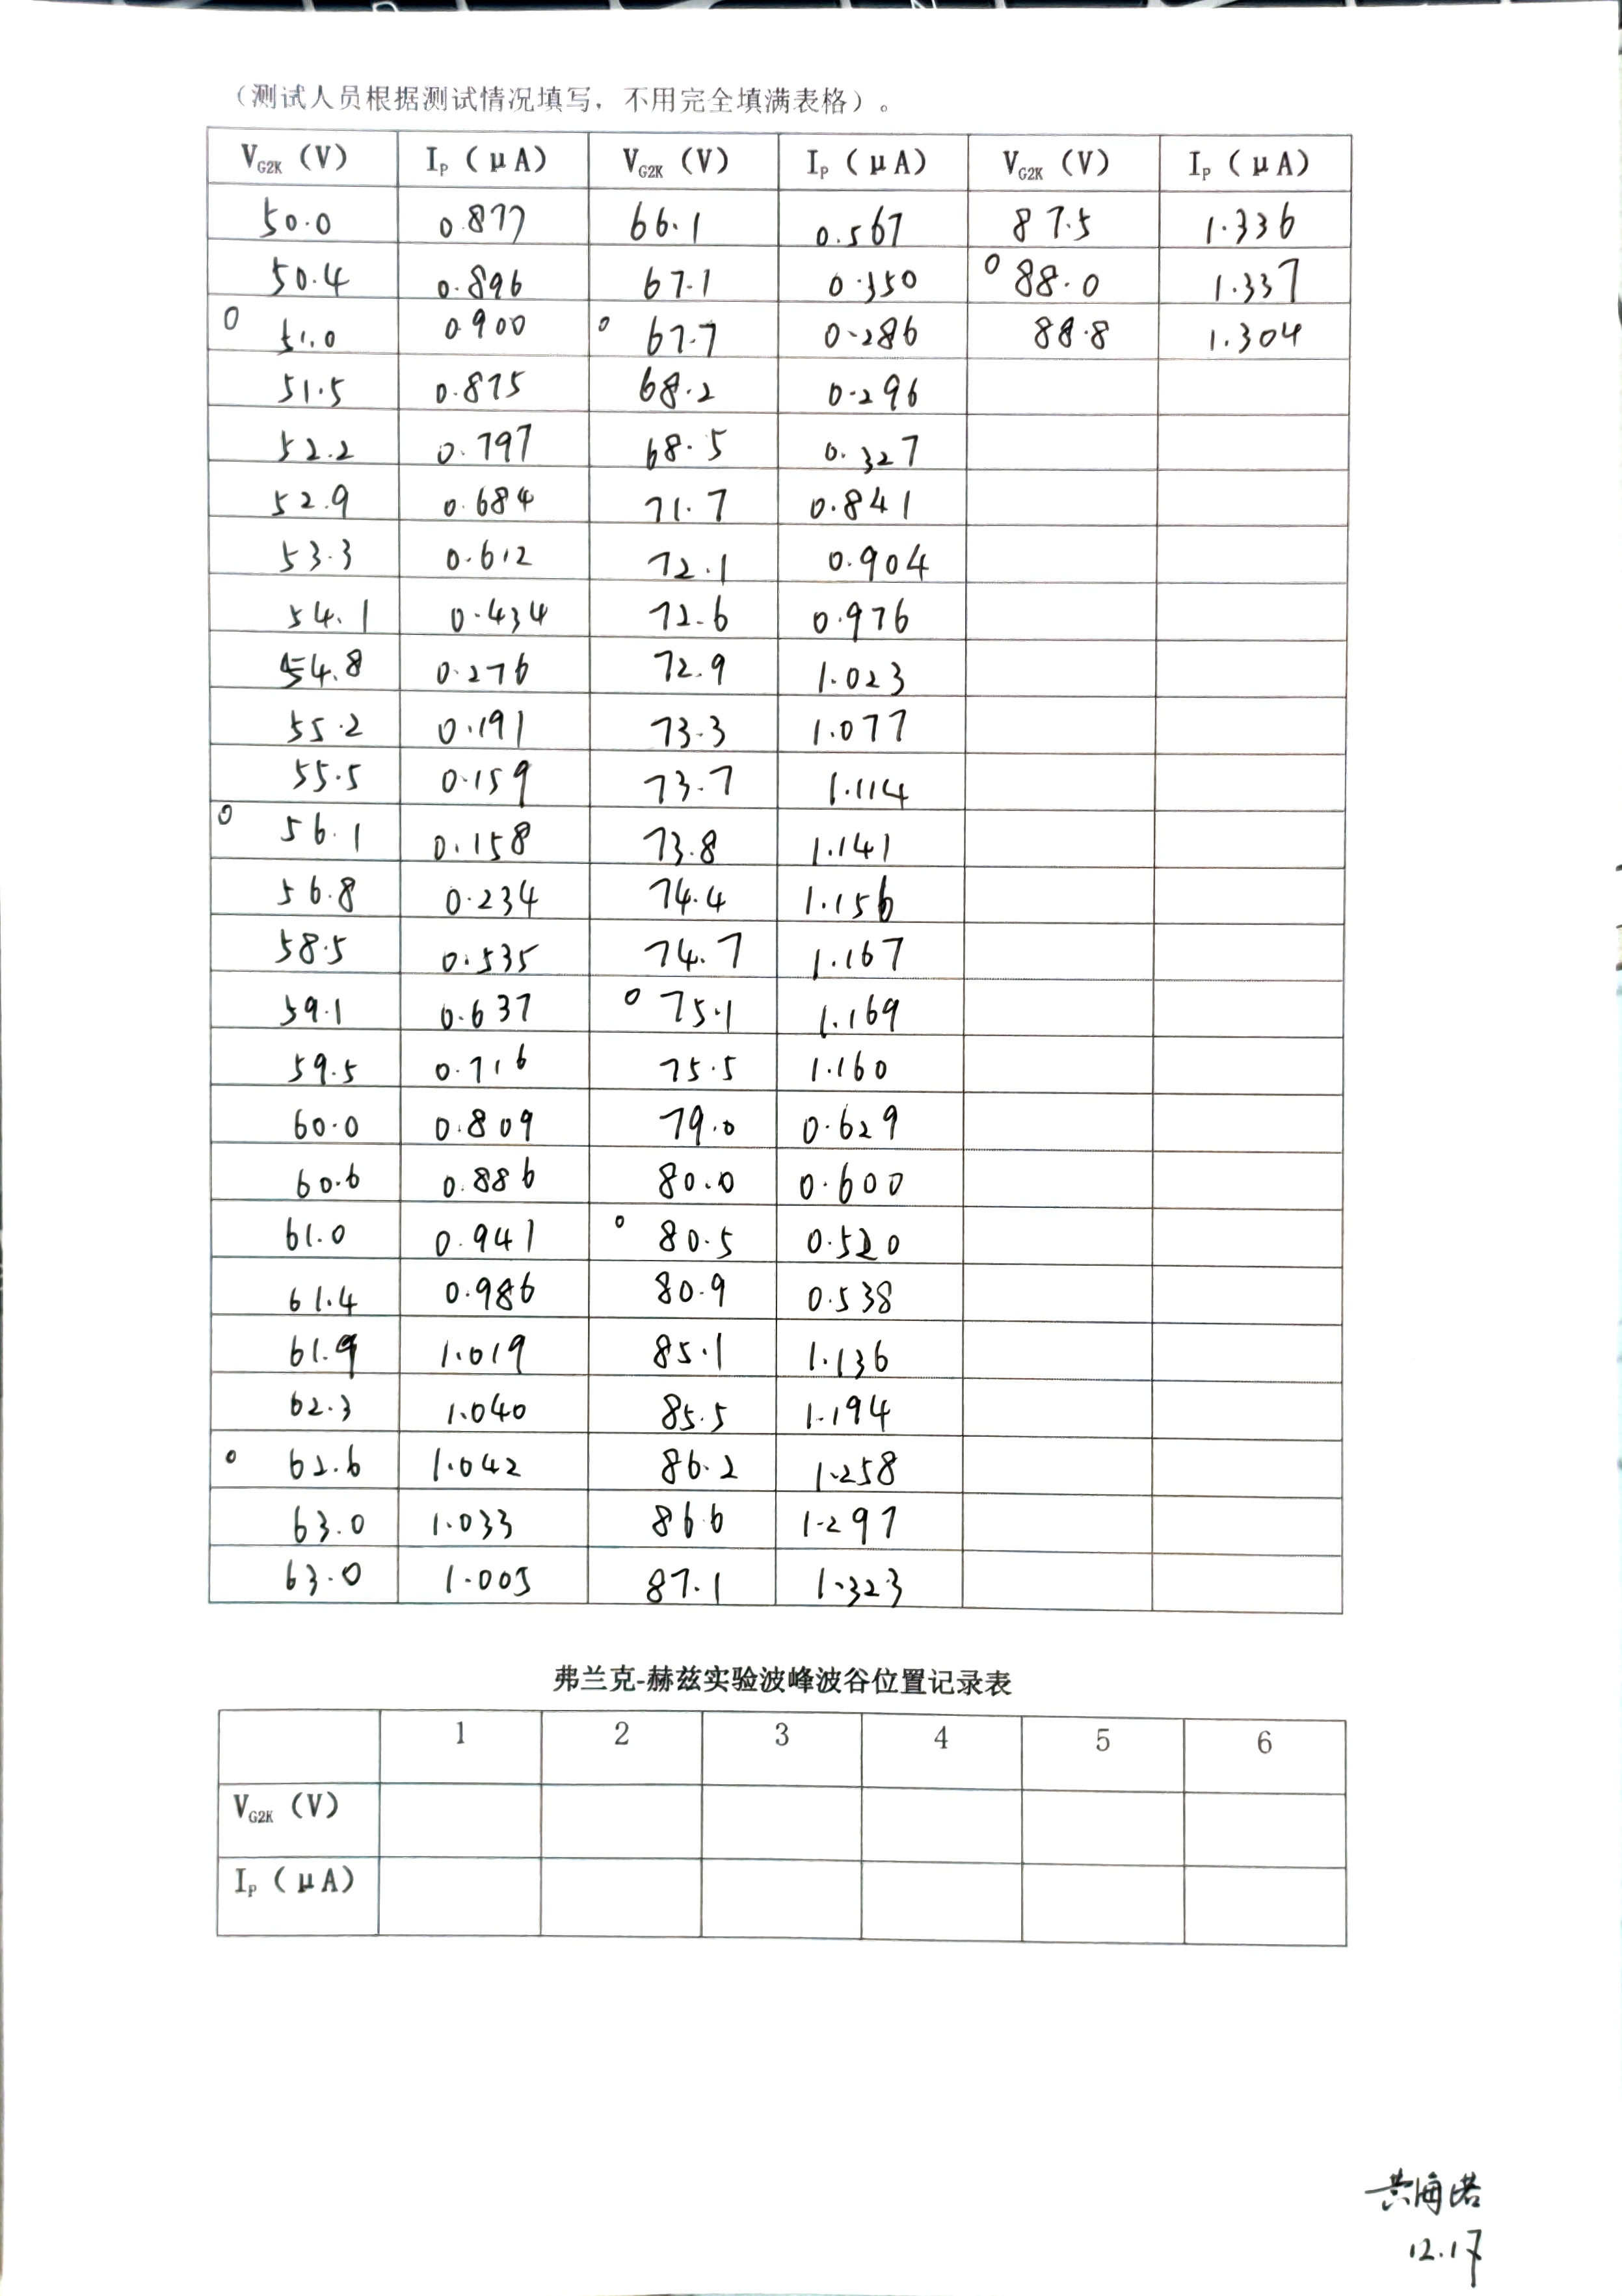
\includegraphics[width=0.9\textwidth]{report5.jpg}
    \caption{原始记录表页码4}
    \label{fig:original_record_5}
\end{figure}

\section{附录：实验数据处理代码}

\subsection{电偏转灵敏度计算与绘图 (calculate\_sensitivity.py)}
\begin{lstlisting}[language=Python]
import matplotlib.pyplot as plt
import numpy as np

# Data extraction from the table
data = {
    "600V_X": {
        "U": np.array([4.9, 8.0, 12.3, 16.4, 20.5, 27.1, 0, 33.6, 40.6, -7.0, -13.5, -20.9, -27.1]),
        "D": np.array([4, 5.5, 9, 12, 15, 20, 0, 25, 30, -5, -10, -15, -20])
    },
    "600V_Y": {
        "U": np.array([-4.6, -9.6, -14.2, -19.1, -23.7, -28.3, 0, 4.8, 9.4, 14.0, 18.2, 22.5, 26.6]),
        "D": np.array([-5, -10, -15, -20, -25, -30, 0, 5, 10, 15, 20, 25, 30])
    },
    "700V_X": {
        "U": np.array([7.6, 15.8, 23.0, 31.2, 38.8, 46.6, 0, -8.0, -15.8, -23.9, -30.9, -38.5, -46.7]),
        "D": np.array([5, 10, 15, 20, 25, 30, 0, -5, -10, -15, -20, -25, -30])
    },
    "700V_Y": {
        "U": np.array([-5.8, -11.2, -16.9, -22.2, -27.6, -32.9, 0, 5.2, 10.5, 15.8, 21.0, 25.8, 30.2]),
        "D": np.array([-5, -10, -15, -20, -25, -30, 0, 5, 10, 15, 20, 25, 30])
    }
}

results = {}

# Set up the plot style
plt.figure(figsize=(12, 10))
# Attempt to use a font that supports Chinese, but fallback to default if necessary
plt.rcParams['font.sans-serif'] = ['SimHei', 'Arial Unicode MS', 'Microsoft YaHei', 'DejaVu Sans'] 
plt.rcParams['axes.unicode_minus'] = False

for i, (key, val) in enumerate(data.items()):
    U = val["U"]
    D = val["D"]
    
    # Linear regression (degree 1)
    slope, intercept = np.polyfit(U, D, 1)
    results[key] = slope
    
    # Plot
    plt.subplot(2, 2, i+1)
    plt.scatter(U, D, label='Data', color='blue', marker='o')
    
    # Create points for line
    x_line = np.linspace(min(U), max(U), 100)
    y_line = slope * x_line + intercept
    
    plt.plot(x_line, y_line, color='red', linestyle='--', label=f'Fit: k={slope:.4f}')
    
    title_parts = key.split('_')
    voltage = title_parts[0]
    direction = title_parts[1]
    
    plt.title(f'Anode Voltage {voltage} - {direction} Direction')
    plt.xlabel('Deflection Voltage U (V)')
    plt.ylabel('Deflection D (mm)')
    plt.legend()
    plt.grid(True, linestyle=':', alpha=0.6)

plt.tight_layout()
output_path = 'deflection_plots.png'
plt.savefig(output_path)
print(f"Plots saved to {output_path}")

print("Calculated Sensitivities (Slope k = D/U):")
for key, val in results.items():
    print(f"{key}: {val:.4f} mm/V")
\end{lstlisting}

\subsection{磁偏转灵敏度计算与绘图 (calculate\_magnetic\_sensitivity.py)}
\begin{lstlisting}[language=Python]
import matplotlib.pyplot as plt
import numpy as np

# Data extraction from the table
# Note: Corrected the likely typo in 700V data (39 -> -39 for -5mm deflection)
data = {
    "600V": {
        "I": np.array([39, 79, 124, 167, 206, 245, 0, -41, -86, -128, -173, -216, -257]),
        "D": np.array([5, 10, 15, 20, 25, 30, 0, -5, -10, -15, -20, -25, -30])
    },
    "700V": {
        "I": np.array([37, 77, 114, 155, 192, 228, 0, -39, -78, -119, -159, -200, -238]),
        "D": np.array([5, 10, 15, 20, 25, 30, 0, -5, -10, -15, -20, -25, -30])
    }
}

results = {}

# Set up the plot style
plt.figure(figsize=(12, 5))
# Attempt to use a font that supports Chinese
plt.rcParams['font.sans-serif'] = ['SimHei', 'Arial Unicode MS', 'Microsoft YaHei', 'DejaVu Sans'] 
plt.rcParams['axes.unicode_minus'] = False

for i, (key, val) in enumerate(data.items()):
    I = val["I"]
    D = val["D"]
    
    # Linear regression (degree 1)
    slope, intercept = np.polyfit(I, D, 1)
    results[key] = slope
    
    # Plot
    plt.subplot(1, 2, i+1)
    plt.scatter(I, D, label='Data', color='blue', marker='o')
    
    # Create points for line
    x_line = np.linspace(min(I), max(I), 100)
    y_line = slope * x_line + intercept
    
    plt.plot(x_line, y_line, color='red', linestyle='--', label=f'Fit: k={slope:.4f}')
    
    plt.title(f'Anode Voltage {key}')
    plt.xlabel('Deflection Current I (mA)')
    plt.ylabel('Deflection D (mm)')
    plt.legend()
    plt.grid(True, linestyle=':', alpha=0.6)

plt.tight_layout()
output_path = 'magnetic_deflection_plots.png'
plt.savefig(output_path)
print(f"Plots saved to {output_path}")

print("Calculated Sensitivities (Slope k = D/I):")
for key, val in results.items():
    print(f"{key}: {val:.4f} mm/mA")
\end{lstlisting}

\subsection{电聚焦数据处理 (calculate\_focusing\_v2.py)}
\begin{lstlisting}[language=Python]
import matplotlib.pyplot as plt
import numpy as np
from scipy import stats

# Data from the LaTeX table
V2 = np.array([600, 650, 700, 750, 800, 850, 900, 950, 1000])
V1 = np.array([133, 137, 142, 153, 164, 170, 180, 191, 198])

# Calculate ratios
ratios = V2 / V1

# Linear regression V1 vs V2
slope, intercept, r_value, p_value, std_err = stats.linregress(V2, V1)
r_squared = r_value**2

# Plotting
plt.figure(figsize=(8, 6))
plt.scatter(V2, V1, color='blue', label='Experimental Data')
plt.plot(V2, slope * V2 + intercept, color='red', linestyle='--', label=f'Linear Fit: $V_1 = {slope:.4f} V_2 {intercept:+.2f}$\n$R^2 = {r_squared:.4f}$')

plt.xlabel(r'Anode Voltage $V_2$ (V)')
plt.ylabel(r'Focusing Voltage $V_1$ (V)')
plt.title(r'Relationship between Focusing Voltage $V_1$ and Anode Voltage $V_2$')
plt.legend()
plt.grid(True)
plt.tight_layout()

# Save plot
plt.savefig('focusing_plot.png', dpi=300)

# Output for LaTeX
print("Ratios:", ", ".join([f"{r:.2f}" for r in ratios]))
print(f"Average Ratio: {np.mean(ratios):.2f}")
print(f"Std Dev of Ratio: {np.std(ratios):.4f}")
print(f"Slope: {slope:.4f}")
print(f"Intercept: {intercept:.4f}")
print(f"R-squared: {r_squared:.4f}")
print(f"Standard Error: {std_err:.4f}")
print(f"Pearson Correlation: {r_value:.4f}")

# Generate LaTeX table row for ratios
ratio_row = " & ".join([f"{r:.2f}" for r in ratios])
print(f"LaTeX Ratio Row: {ratio_row}")
\end{lstlisting}

\subsection{弗兰克-赫兹实验数据处理 (process\_fh\_data.py)}
\begin{lstlisting}[language=Python]
import numpy as np
import matplotlib.pyplot as plt
from scipy.signal import find_peaks
from scipy.stats import linregress

# Data from the LaTeX table
data_str = """
2.2  0.034
5.4  0.033
10.5 0.038
12.5 0.091
13.3 0.114
14.2 0.144
15.2 0.169
16.2 0.197
16.9 0.215
17.4 0.227
17.7 0.232
18.1 0.239
18.4 0.243
18.6 0.245
18.8 0.248
19.0 0.248
19.2 0.246
19.6 0.243
19.8 0.237
20.8 0.204
21.1 0.192
21.6 0.174
21.8 0.166
22.2 0.152
22.5 0.148
22.8 0.153
23.0 0.160
23.7 0.202
24.6 0.286
25.6 0.384
26.4 0.453
27.1 0.487
27.8 0.517
28.0 0.519
28.2 0.518
28.4 0.517
28.8 0.513
29.1 0.500
30.9 0.347
31.5 0.267
32.0 0.198
32.4 0.154
32.6 0.134
33.0 0.112
33.4 0.112
33.6 0.123
34.0 0.157
35.8 0.413
36.2 0.470
37.0 0.580
37.4 0.604
37.7 0.646
38.0 0.671
38.4 0.700
38.5 0.694
38.7 0.711
39.0 0.724
39.5 0.727
39.9 0.716
40.1 0.704
41.9 0.457
42.6 0.326
43.2 0.200
43.6 0.134
43.9 0.103
44.2 0.092
44.4 0.096
44.4 0.100
44.6 0.119
45.0 0.151
46.9 0.480
48.1 0.709
48.4 0.732
49.0 0.808
49.6 0.868
50.0 0.877
50.4 0.896
51.0 0.900
51.5 0.875
52.2 0.797
52.9 0.684
53.3 0.612
54.1 0.434
54.8 0.276
55.2 0.191
55.5 0.159
56.1 0.158
56.8 0.234
58.5 0.535
59.1 0.637
59.5 0.716
60.0 0.809
60.6 0.886
61.0 0.941
61.4 0.986
61.9 1.019
62.3 1.040
62.6 1.042
63.0 1.033
63.0 1.005
66.1 0.567
67.1 0.350
67.7 0.286
68.2 0.296
68.5 0.327
71.7 0.841
72.1 0.904
72.6 0.976
72.9 1.023
73.3 1.077
73.7 1.114
73.8 1.141
74.4 1.156
74.7 1.167
75.1 1.169
75.5 1.160
79.0 0.629
80.0 0.600
80.5 0.520
80.9 0.538
85.1 1.136
85.5 1.194
86.2 1.258
86.6 1.297
87.1 1.323
87.5 1.336
88.0 1.337
88.8 1.304
"""

data = []
for line in data_str.strip().split('\n'):
    parts = line.split()
    if len(parts) == 2:
        data.append([float(parts[0]), float(parts[1])])

data = np.array(data)
V = data[:, 0]
I = data[:, 1]

# Find peaks
peaks, _ = find_peaks(I, distance=5, prominence=0.02) 

# Find valleys (invert I)
valleys, _ = find_peaks(-I, distance=5, prominence=0.05)

print("Peaks indices:", peaks)
print("Valleys indices:", valleys)

peak_V = V[peaks]
peak_I = I[peaks]
valley_V = V[valleys]
valley_I = I[valleys]

print("Peaks (V, I):")
for v, i in zip(peak_V, peak_I):
    print(f"{v}, {i}")

print("\nValleys (V, I):")
for v, i in zip(valley_V, valley_I):
    print(f"{v}, {i}")

# Plotting
plt.figure(figsize=(10, 6))
plt.plot(V, I, '-o', markersize=3, label='Experimental Data')
plt.plot(peak_V, peak_I, 'rx', markersize=8, label='Peaks')
plt.plot(valley_V, valley_I, 'bx', markersize=8, label='Valleys')
plt.xlabel(r'$V_{G2K}$ (V)')
plt.ylabel(r'$I_p$ ($\mu$A)')
plt.title(r'Frank-Hertz Experiment $I_p - V_{G2K}$ Curve')
plt.legend()
plt.grid(True)
plt.savefig('fh_plot.png')

# Analysis
# Linear regression for peaks
peak_n = np.arange(1, len(peak_V) + 1)
slope_p, intercept_p, r_value_p, p_value_p, std_err_p = linregress(peak_n, peak_V)

# Linear regression for valleys
valley_n = np.arange(1, len(valley_V) + 1)
slope_v, intercept_v, r_value_v, p_value_v, std_err_v = linregress(valley_n, valley_V)

avg_slope = (slope_p + slope_v) / 2
theory_argon = 11.55
error = abs(avg_slope - theory_argon) / theory_argon * 100

print("\nAnalysis Results:")
print(f"Peaks Regression: slope={slope_p:.4f}, intercept={intercept_p:.4f}, R2={r_value_p**2:.4f}")
print(f"Valleys Regression: slope={slope_v:.4f}, intercept={intercept_v:.4f}, R2={r_value_v**2:.4f}")
print(f"Average Excitation Potential: {avg_slope:.4f} V")
print(f"Error vs Argon (11.55V): {error:.2f}%")
\end{lstlisting}

\end{document}